\documentclass[12pt,a4paper]{article}

% ===== Packages =====
\usepackage[utf8]{inputenc}
\usepackage[T1]{fontenc}
\usepackage{lmodern}
\usepackage[margin=1in]{geometry}
\usepackage{amsmath,amssymb,amsthm}
\usepackage{mathtools}
\usepackage{booktabs}
\usepackage{tabularx}
\usepackage{longtable}
\usepackage{array}
\usepackage{multirow}
\usepackage{graphicx}
\usepackage{float}
\usepackage{caption}
\usepackage{subcaption}
\usepackage[colorlinks=true,linkcolor=blue,citecolor=blue,urlcolor=blue]{hyperref}
\usepackage{natbib}
\usepackage{setspace}
\usepackage{parskip}
\usepackage{microtype}
\usepackage{xcolor}
\usepackage{threeparttable}
\usepackage{siunitx}
\usepackage{rotating}
\usepackage{pdflscape}
\usepackage{enumitem}
\usepackage{appendix}
\usepackage{titlesec}
\usepackage{abstract}
\usepackage{tikz}
\usepackage{pgfplots}
\pgfplotsset{compat=1.18}
\usepgfplotslibrary{groupplots}

% ===== Theorem environments =====
\newtheoremstyle{predstyle}
  {0.5em}{0.5em}{\normalfont}{}{\bfseries}{.}{ }{}
\theoremstyle{predstyle}
\newtheorem{prediction}{Prediction}
\newtheorem{proposition}{Proposition}
\newtheorem{assumption}{Assumption}
\theoremstyle{plain}

% ===== Line spacing =====
\doublespacing

% ===== CER/Elsevier-style manuscript formatting =====
\setcounter{secnumdepth}{3}
\setcounter{tocdepth}{3}
\titleformat{\section}{\normalfont\large\bfseries}{\thesection.}{0.6em}{}
\titleformat{\subsection}{\normalfont\normalsize\bfseries}{\thesubsection.}{0.6em}{}
\titleformat{\subsubsection}{\normalfont\normalsize\itshape}{\thesubsubsection.}{0.6em}{}

% ===== Custom commands =====
\newcommand{\SMI}{\mathrm{SMI}}
\newcommand{\AI}{\mathrm{AI}}
\newcommand{\IV}{\mathrm{IV}}
\newcommand{\Overedu}{\mathit{Overedu}}
\newcommand{\Emp}{\mathit{Emp}}
\newcommand{\Jmr}{\mathit{Jmr}}
\newcommand{\Edq}{\mathit{Edq}}
\newcommand{\Nfc}{\mathit{Nfc}}

\begin{document}

\begin{center}
{\large\bfseries Artificial Intelligence, Skill Mismatch, and Employment Reallocation in China\par}
\vspace{0.8em}
{\normalsize Wang Weijia\par}
\vspace{0.2em}
{\small School of Economics and Finance, Xi'an Jiaotong University\par}
{\small \texttt{18522704823@163.com}\par}
\end{center}

\begin{abstract}
This paper asks whether firm-level AI adoption creates inclusive employment gains in China and how pre-existing skill mismatch shapes the answer. Using panel data on 10,563 firm-year observations for Chinese A-share listed firms from 2010 to 2022, I combine annual-report text measures of AI adoption with firm employment structure and overeducation measures. Instrumental-variable estimates use an education-expansion shift-share design and leave-one-out peer AI diffusion, supplemented by a Broadband China difference-in-differences validation. AI adoption raises total employment (IV coefficient: 0.574) and increases the high-skilled labor share by 0.109, while reducing the low-skilled share by 0.150. Overeducation weakens AI's complementarity with high-skilled labor but buffers low-skilled workers from displacement. Within the task-based framework, these employment shifts imply a widening of the skill wage premium; annual-report pay dispersion data provide direct evidence consistent with this channel---AI adoption is associated with a wider within-firm compensation gap (IV coefficient: 0.031), an effect that overeducation compresses by reducing the effective productivity of credential holders at AI-complementary task margins. The findings show that AI creates jobs and income opportunities unevenly, and that the conditions governing this unevenness---credential-task alignment, industry mismatch, and local labor-market institutions---determine whether AI adoption widens or contains inequality in labor-market outcomes.
\end{abstract}

\noindent\textbf{Keywords:} artificial intelligence; skill mismatch; overeducation; employment structure; China; instrumental variables.

\noindent\textbf{JEL classification:} J23; J24; J31; O33; C26.

\vspace{0.5em}

% ============================================================
\section{Introduction}
\label{sec:intro}
% ============================================================

China's labor market faces a distinctive tension. The number of college graduates has risen sharply, from roughly 1.1 million in 2000 to over 11 million in 2023 \citep{moe2024}. Digital and manufacturing firms simultaneously report persistent shortages of applied technical workers \citep{ilo2020skills}. Many young graduates enter jobs that do not use their education, while other workers lack the cognitive and technical skills that rapidly automating firms need. These pressures arise against a backdrop of rising wage inequality that has attracted sustained attention since the early reform era \citep{knight2003, knight2014}: the returns to education in China have shifted considerably over the past three decades, and technology adoption is one of the forces driving that shift. In this setting, the central question about artificial intelligence is not simply whether it destroys jobs, nor simply whether it raises wages on average. The more relevant question is whether AI creates employment and earnings opportunities that match workers' skills, and how pre-existing mismatch determines who captures the gains \citep{brynjolfsson2014second}.

This paper estimates how firm-level AI adoption affects employment quantity and skill composition in China, and how pre-existing overeducation and skill mismatch condition these effects. The analysis uses panel data on Chinese A-share listed firms from 2010 to 2022. AI adoption is measured from firms' annual reports using AI-related text, including terms such as artificial intelligence, machine learning, deep learning, and large language models. The main outcomes are total employment, the share of employees with a bachelor's degree or above (high-skilled), and the share of employees with high-school education or below (low-skilled). The key moderator is firm-level overeducation, defined as the excess of workers' actual education over the education typically required by the jobs they hold. I also use an industry-level skill mismatch index to test whether broader labor-market mismatch weakens AI's employment effect.

The main empirical challenge is selection into AI adoption. Better-managed firms with stronger human-capital reserves may both adopt AI earlier and expand employment faster, so raw correlations confound AI adoption with firm quality. The paper addresses this concern using two sources of variation. The primary instrument is an education-expansion shift-share design (Edushock), which interacts the 1999 higher education expansion with baseline industry reliance on college-educated labor. This instrument drives variation in overeducation exposure across industries and years without directly entering firms' employment decisions, conditional on fixed effects and controls. The secondary instrument is leave-one-out peer AI adoption among other firms in the same industry-region-year cell, which captures local AI diffusion pressure. A difference-in-differences design based on the Broadband China pilot policy provides complementary evidence from an independent infrastructure shock.

The first result is that AI raises total employment after correcting for endogeneity. The OLS coefficient on AI is \(-0.012\), consistent with negative selection: firms under employment pressure may discuss AI more. After instrumenting, the IV-2SLS coefficient rises to \(0.574\), significant at the 1 percent level. The sign reversal reflects upward bias correction: causal variation in AI adoption increases labor demand through productivity and new-task channels. Overeducation dampens this gain: the interaction \(AI \times \Overedu\) is \(-0.066\), implying that a one-unit increase in overeducation reduces AI's marginal employment effect by about 11.5 percent.

The second result is that AI reallocates jobs across skill groups. IV estimates show that AI increases the high-skilled labor share by \(0.109\) and reduces the low-skilled share by \(0.150\). Overeducation weakens high-skill complementarity (interaction coefficient \(-0.244\)) while cushioning low-skill displacement (interaction coefficient \(0.271\)). These two signs together describe the dual face of excess education: it traps workers in credential-heavy but AI-exposed roles, yet also provides general human capital that helps workers avoid the most routine displaced jobs.

The third result is that institutions shape the returns to AI. An industry skill mismatch index negatively moderates AI's employment effect, with an interaction coefficient of \(-0.004\). Better employment matching mitigates the adverse interaction between AI and overeducation. General higher education quality can paradoxically amplify mismatch when it expands academic credentials without aligning them with industry task demand.

The fourth result connects employment reallocation to income distribution directly. Using the log ratio of executive compensation to average employee wages as a within-firm measure of pay dispersion, AI adoption is associated with a widening of the within-firm compensation gap (IV coefficient: \(0.031\)). The overeducation moderator compresses this effect, with an interaction coefficient of \(-0.018\), consistent with the theoretical prediction that credential-task misalignment reduces the effective productivity of higher-tier workers in AI-complementary tasks. These findings situate the employment results within the broader literature on wage inequality and labor-market transition in China \citep{knight2003, knight2014}.

The paper contributes to three literatures. First, it adds firm-level evidence on automation, task-biased technological change, and labor demand \citep{autor2003skill, autor2018automation, goos2007lousy, goos2014explaining, acemoglu2018artificial, acemoglu2020robots, acemoglu2022tasks, acemoglu2026automation}. Rather than asking only whether technology substitutes for labor, it shows how AI changes total employment and the skill mix inside Chinese firms, derives from the task model the implied direction of change in the skill wage premium, and provides direct firm-level evidence on pay dispersion that is consistent with these distributional predictions. Second, it connects this literature with research on overeducation and skill mismatch \citep{mcguinness2006overeducation, pellizzari2017new}. The results show that mismatch is not merely an outcome of labor-market adjustment; it is a state variable that governs whether AI adoption generates inclusive employment and earnings gains. Third, the paper contributes to the empirical literature on income distribution and labor-market adjustment in China. Research in this tradition has documented how education returns, wage gaps, and employment structure have evolved through China's transition \citep{knight2003, knight2014}. The present paper extends that agenda by examining how a new wave of technology adoption interacts with the educational mismatches that accumulated during rapid credential expansion, shaping the distributive consequences of AI for workers at different points in the skill distribution.

The rest of the paper proceeds as follows. Section~\ref{sec:framework} develops a task-based conceptual framework. Section~\ref{sec:data} describes the data and variable construction. Section~\ref{sec:strategy} presents the empirical strategy. Section~\ref{sec:results} reports the main estimates, including a direct analysis of within-firm pay dispersion. Section~\ref{sec:robust} presents robustness checks. Section~\ref{sec:concl} concludes.

% ============================================================
\section{Conceptual Framework}
\label{sec:framework}
% ============================================================

\subsection{Tasks, AI Adoption, and Employment}

The framework starts from the task approach to technological change \citep{autor2003skill, acemoglu2018artificial, acemoglu2022tasks}. Firms produce output by combining tasks that differ in complexity. AI adoption lowers the cost of performing some tasks with capital and software, creating a displacement force for workers assigned to automatable routine tasks. It also creates a productivity and reinstatement force when AI raises output, expands demand, and opens new human-machine complementary tasks \citep{aghion1992model, acemoglu2022tasks}.

Let \(Y_{it}\) denote firm \(i\)'s employment outcome in year \(t\). The outcome can be total employment, the high-skilled employment share, or the low-skilled employment share. AI adoption affects \(Y_{it}\) through two channels:
\[
\frac{\partial Y_{it}}{\partial AI_{it}}
= \underbrace{\frac{\partial Y_{it}^{new}}{\partial AI_{it}}}_{\text{new-task and scale effects}}
- \underbrace{\frac{\partial Y_{it}^{auto}}{\partial AI_{it}}}_{\text{automation displacement}}.
\]
The sign of the total effect is ambiguous ex ante. If AI mainly expands output and creates complementary tasks, total employment rises. If automation displacement dominates, employment falls. For China's listed firms, which are relatively large and more likely to reorganize tasks internally, the productivity and new-task channels may dominate for total employment, while displacement may remain concentrated in low-skilled labor.

\begin{prediction}[Total employment]
\label{pred:total}
AI adoption increases total employment when productivity and new-task effects dominate displacement. The effect is smaller when pre-existing skill mismatch prevents workers from moving into AI-complementary tasks. This prediction maps to Table~\ref{tab:empbase}.
\end{prediction}

\subsection{Overeducation and Skill Composition}

Overeducation captures a mismatch between workers' educational attainment and the requirements of jobs they hold. It can help or hurt adjustment to AI through two channels. On one side, workers with more education may have greater learning capacity and can move out of routine jobs more easily, softening low-skilled displacement \citep{becker1964human}; this is the human-capital buffer channel. On the other side, excess credentials without task-specific AI skills create redundancy: highly educated workers may be concentrated in tasks that AI can partially perform, and their training does not map into the new tasks firms need \citep{spence1973job}; this is the skill-redundancy trap.

The sign of \(AI_{it} \times \Overedu_{it}\) therefore depends on the outcome variable. For total and high-skilled employment, overeducation can weaken AI's complementary effect when educated workers are not matched to AI-complementary tasks. For low-skilled employment, overeducation may soften displacement when general human capital helps workers transition across tasks.

\begin{prediction}[Overeducation as moderator]
\label{pred:overedu}
Overeducation reduces the positive effect of AI on total and high-skilled employment when credentials are poorly aligned with task demand. It reduces low-skill displacement when general human capital helps workers move across tasks. This prediction maps to Tables~\ref{tab:empbase} and~\ref{tab:skillstructure}.
\end{prediction}

\subsection{Institutional and Industry Buffers}

The adjustment cost from AI adoption depends on institutions and industry task demand. Higher employment matching rates signal better alignment between education and jobs. Stronger industry-university-research cooperation reduces the gap between training content and firm needs. Industry cognitive skill demand determines whether AI functions mainly as an augmenting tool or a substitute for routine labor. Education quality has an ambiguous effect: it improves learning capacity, but if it expands academic credentials without applied AI-complementary skills, it may deepen rather than reduce mismatch.

\begin{prediction}[Mismatch and institutional buffers]
\label{pred:buffers}
Industry skill mismatch weakens AI's employment gains. Better job matching and stronger industry-university-research cooperation mitigate the adverse interaction between AI and overeducation, while education quality disconnected from industry demand worsens mismatch. This prediction maps to Tables~\ref{tab:mechanisms} and~\ref{tab:smi}.
\end{prediction}

\subsection{Task Reallocation, the Skill Wage Premium, and Income Distribution}
\label{sec:wage_theory}

The employment reallocation predictions of the task model carry direct implications for income distribution, and situating these implications explicitly is important for understanding the stakes of the analysis. Research on China's labor market has documented that the returns to education and the wage gap between skill groups have shifted substantially since the early reform period \citep{knight2003, knight2014}. Technology adoption is one of the mechanisms through which such shifts occur. The task model provides a framework for deriving the direction of that mechanism from the employment evidence presented in this paper.

In a competitive labor market where workers earn the marginal product of their labor across the tasks they perform, the equilibrium wage of a worker of type $\theta$ in firm $i$ is proportional to:
\[
w_{\theta,it} \;\propto\; \int_{T_\theta(AI_{it})} A_\theta(x)\, dx,
\]
where $T_\theta(AI_{it})$ is the set of tasks allocated to type $\theta$ given the firm's AI adoption level and $A_\theta(x)$ is effective labor productivity in task $x$. When AI adoption expands the set of high-skill complementary tasks and contracts the set of routine tasks, two wage effects operate in tandem. High-skilled workers' productivity at the new task margin rises, pushing up $w_{h,it}$; low-skilled workers face a deteriorating outside option as automated tasks disappear, compressing $w_{l,it}$ or reducing their employment probability. The skill premium $\pi_{it} = w_{h,it}/w_{l,it}$ therefore satisfies
\[
\frac{\partial \ln \pi_{it}}{\partial AI_{it}} > 0
\]
under the same conditions that generate the employment reallocation in Predictions~\ref{pred:total} and~\ref{pred:overedu}. In this sense the employment share results are a sufficient statistic for the direction of AI's effect on within-firm wage inequality, given an estimated skill premium.

Overeducation modulates this distributional channel through its effect on effective productivity. In the tradition of \citet{nelson1966investment}, the ability to absorb and implement new technologies depends on the match between workers' education and the cognitive demands of those technologies. When a worker's credentials exceed the requirements of available AI-complementary tasks, $A_h(x)$ at the new task margin is lower than it would be for a correctly matched worker, because the worker's training is misaligned with the specific cognitive demands of those tasks. This reduces the wage gain attributable to AI adoption, so that:
\[
\frac{\partial^2 \ln \pi_{it}}{\partial AI_{it}\, \partial \Overedu_{it}} < 0.
\]
Overeducation thus compresses the skill premium that AI adoption would otherwise generate. This is the income distribution analogue of the employment finding that overeducation weakens AI's complementarity with high-skilled labor: the mechanism is the same mismatch between credentials and task demand, operating on wages rather than headcounts.

\begin{prediction}[Skill wage premium and income distribution]
\label{pred:wage}
AI adoption raises the within-firm skill wage premium under conditions of positive high-skill complementarity and low-skill displacement. Overeducation compresses this distributional effect by reducing effective productivity at the AI-complementary task margin. Industry skill mismatch amplifies dispersion in returns when it concentrates displacement on low-skilled workers without providing reallocation channels. This prediction extends Predictions~\ref{pred:total}--\ref{pred:buffers} to income distribution consequences and maps to Table~\ref{tab:wageprem} and the discussion in Section~\ref{sec:concl}.
\end{prediction}

Figure~\ref{fig:taskspace} summarises the mechanism. The upper bar shows task allocation before AI adoption, divided into routine low-skill tasks (left) and non-routine high-skill tasks (right). The lower bar shows the post-AI allocation: a subset of routine tasks is automated, reducing low-skill task variety and putting downward pressure on $w_L$; new AI-complementary tasks are created at the high-complexity margin, raising $w_H$. The box at the bottom of the figure captures the overeducation moderating channel: when workers' credentials exceed task requirements, their effective productivity $A_h(x)$ at the new-task margin is reduced, compressing the resulting skill premium.

\begin{figure}[H]
\centering
\resizebox{\linewidth}{!}{%
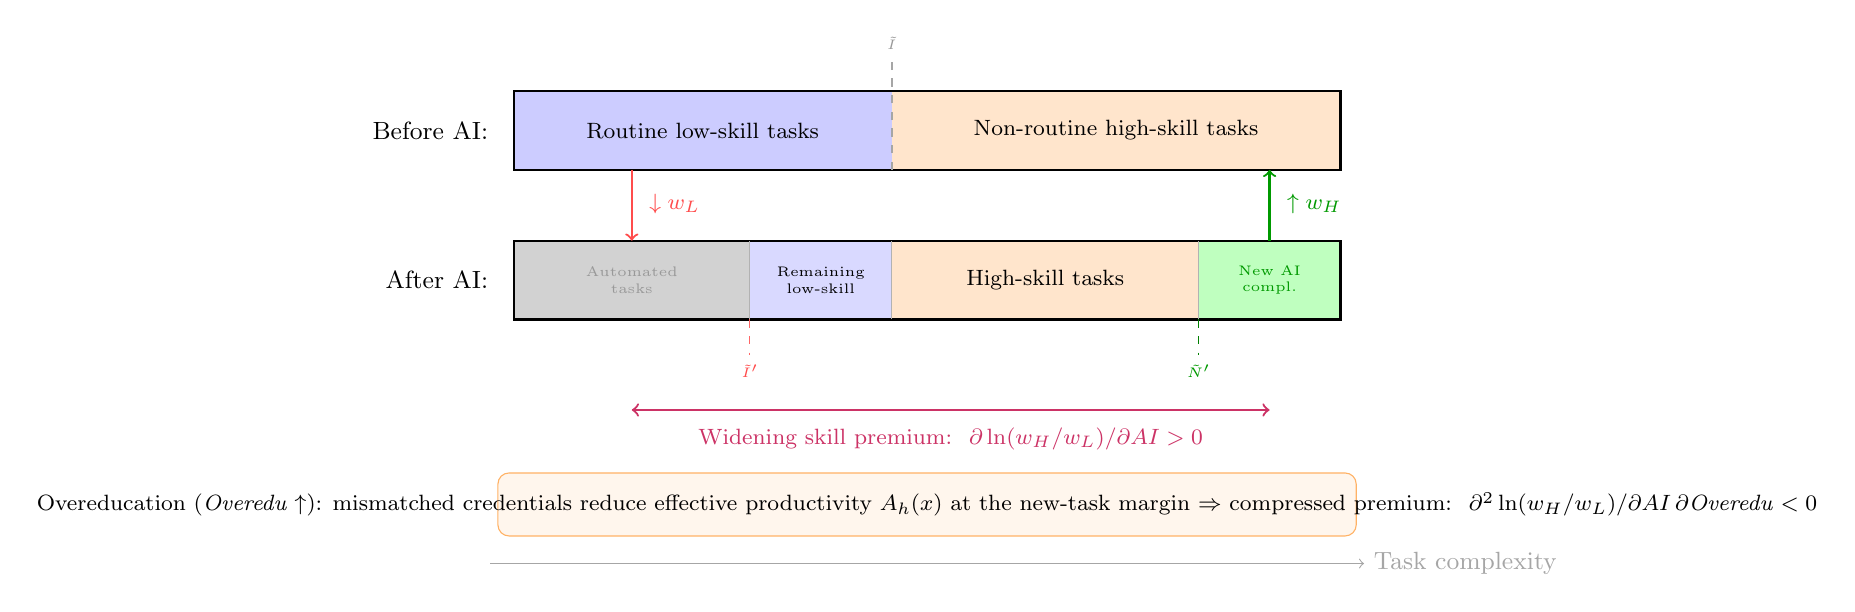
\begin{tikzpicture}

% ---- BEFORE AI ----
\node[anchor=east, font=\small] at (-0.2, 1.2) {Before AI:};
\fill[blue!20] (0, 0.7) rectangle (4.8, 1.7);
\node[font=\footnotesize] at (2.4, 1.2) {Routine low-skill tasks};
\fill[orange!20] (4.8, 0.7) rectangle (10.5, 1.7);
\node[font=\footnotesize] at (7.65, 1.2) {Non-routine high-skill tasks};
\draw[thick] (0,0.7) rectangle (10.5,1.7);
\draw[gray!70, thick, dashed] (4.8,0.7) -- (4.8,2.1);
\node[font=\tiny, gray!80, above] at (4.8,2.1) {$\tilde{I}$};

% ---- AFTER AI ----
\node[anchor=east, font=\small] at (-0.2, -0.7) {After AI:};
\fill[gray!35] (0, -1.2) rectangle (3.0, -0.2);
\node[font=\tiny, text=gray!80, align=center] at (1.5, -0.7) {Automated\\tasks};
\fill[blue!15] (3.0, -1.2) rectangle (4.8, -0.2);
\node[font=\tiny, align=center] at (3.9, -0.7) {Remaining\\low-skill};
\fill[orange!20] (4.8, -1.2) rectangle (8.7, -0.2);
\node[font=\footnotesize] at (6.75, -0.7) {High-skill tasks};
\fill[green!25] (8.7, -1.2) rectangle (10.5, -0.2);
\node[font=\tiny, align=center, text=green!60!black] at (9.6, -0.7) {New AI\\compl.};
\draw[thick] (0,-1.2) rectangle (10.5,-0.2);
\draw[gray!60] (3.0,-1.2) -- (3.0,-0.2);
\draw[gray!60] (4.8,-1.2) -- (4.8,-0.2);
\draw[gray!60] (8.7,-1.2) -- (8.7,-0.2);

% Threshold labels
\draw[red!60, dashed, thin] (3.0,-1.2) -- (3.0,-1.65);
\node[font=\tiny, red!70, below] at (3.0,-1.65) {$\tilde{I}'$};
\draw[green!50!black, dashed, thin] (8.7,-1.2) -- (8.7,-1.65);
\node[font=\tiny, green!60!black, below] at (8.7,-1.65) {$\tilde{N}'$};

% Wage effect arrows
\draw[->, thick, red!70] (1.5, 0.7) -- (1.5, -0.2);
\node[font=\footnotesize, right, red!70] at (1.6, 0.27) {$\downarrow w_L$};
\draw[->, thick, green!60!black] (9.6, -0.2) -- (9.6, 0.7);
\node[font=\footnotesize, right, green!60!black] at (9.7, 0.27) {$\uparrow w_H$};

% Skill premium arrow
\draw[<->, thick, purple!80] (1.5, -2.35) -- (9.6, -2.35);
\node[font=\footnotesize, purple!80, below] at (5.55, -2.45) {Widening skill premium: $\;\partial \ln(w_H/w_L)/\partial AI > 0$};

% Overeducation moderator box
\draw[rounded corners, draw=orange!60, fill=orange!7] (-0.2,-3.15) rectangle (10.7,-3.95);
\node[font=\footnotesize, align=center] at (5.25, -3.55)
  {Overeducation $(\Overedu\uparrow)$: mismatched credentials reduce effective productivity $A_h(x)$ at the new-task margin $\Rightarrow$ compressed premium: $\;\partial^2 \ln(w_H/w_L)/\partial AI\,\partial\Overedu < 0$};

% Task complexity axis
\draw[->, gray!70] (-0.3, -4.3) -- (10.8, -4.3);
\node[right, gray!70, font=\small] at (10.8,-4.3) {Task complexity};

\end{tikzpicture}%
}
\caption{Task Space Reallocation, Wages, and the Overeducation Channel}
\label{fig:taskspace}
\begin{minipage}{0.92\textwidth}
\footnotesize
Notes: The figure illustrates the mechanism from Section~\ref{sec:wage_theory}. Before AI adoption, tasks are divided into routine low-skill (blue) and non-routine high-skill (orange) segments. AI adoption shifts the automation threshold from $\tilde{I}$ to $\tilde{I}'$, displacing some routine tasks, and creates new AI-complementary tasks at the high-complexity frontier $\tilde{N}'$. The resulting wage effects---$\downarrow w_L$ from displacement and $\uparrow w_H$ from new-task creation---widen the skill premium. Overeducation (orange box) reduces workers' effective productivity at the new-task margin, compressing this distributional effect.
\end{minipage}
\end{figure}

The paper does not estimate wage equations directly, and the empirical strategy focuses on employment structure as the primary outcome. This choice reflects data availability: firm-level employment structure is observable from annual reports, while matched worker wages require data that listed-company disclosures do not provide with the necessary coverage. The theoretical prediction nevertheless establishes that the paper's employment findings are not silent on distributional questions. Because employment shares and wages are jointly determined by the same task-allocation equilibrium, evidence that AI shifts the employment mix toward high-skill workers---while overeducation moderates that shift---is at the same time evidence about the forces shaping skill wage inequality in firms at the frontier of AI adoption in China.

% ============================================================
\section{Data and Measurement}
\label{sec:data}
% ============================================================

\subsection{Data Sources and Sample Construction}

The sample covers Chinese A-share listed companies from 2010 to 2022. After excluding financial firms (SIC codes corresponding to banking, insurance, and securities), ST and *ST firms under special treatment, and observations with missing key variables (AI index, employment structure, or financial controls), the final panel contains 10,563 firm-year observations. The unbalanced panel covers 1,287 distinct firms. Firm financial and governance variables come from CSMAR and Wind. AI adoption is measured from listed-company annual reports obtained through CNRDS. Employment structure is constructed from firms' disclosed employee education categories in annual report notes. Job-education requirements are matched from online job-posting data and industry occupation data. Industry and regional variables are merged from official statistical yearbooks, CFPS-based labor-market measures, and task measures crosswalked from O*NET to Chinese industries using the concordance in \citet{autor2013china}. Table~\ref{tab:sampleconstruction} in Appendix~\ref{app:tables} details the sample construction steps.

Table~\ref{tab:summary} reports descriptive statistics. The average AI index is 0.487, with a standard deviation of 0.612, indicating substantial right skew consistent with a diffusion process where most firms are early adopters. The average log employment is 7.842. The average high-skilled labor share is 32.4 percent and the average low-skilled labor share is 41.7 percent.

\begin{table}[H]
\centering
\caption{Summary Statistics}
\label{tab:summary}
\begin{threeparttable}
\small
\begin{tabular}{lrrrrrr}
\toprule
Variable & Mean & SD & Min & Median & Max & N \\
\midrule
\multicolumn{7}{l}{\textit{Outcomes and mismatch measures}} \\
Skill mismatch index (\(\SMI\)) & 2.340 & 0.410 & 1.270 & 2.310 & 3.620 & 10,563 \\
Overeducation (\(\Overedu\)) & 0.082 & 0.057 & 0.000 & 0.071 & 0.398 & 10,563 \\
Overeducation dispersion & 0.063 & 0.034 & 0.000 & 0.058 & 0.246 & 9,054 \\
\multicolumn{7}{l}{\textit{AI adoption and instruments}} \\
AI adoption index & 0.487 & 0.612 & 0.000 & 0.215 & 4.873 & 10,563 \\
Peer AI adoption instrument & 0.521 & 0.298 & 0.041 & 0.482 & 1.738 & 10,563 \\
Log AI keyword count & 0.853 & 0.974 & 0.000 & 0.693 & 5.214 & 10,563 \\
\multicolumn{7}{l}{\textit{Employment and mechanism variables}} \\
Log total employment & 7.842 & 1.213 & 4.094 & 7.731 & 11.215 & 10,563 \\
High-skilled labor share (\%) & 32.400 & 21.800 & 0.000 & 28.700 & 95.300 & 9,054 \\
Low-skilled labor share (\%) & 41.700 & 24.600 & 0.000 & 39.800 & 96.200 & 9,054 \\
Cognitive skill demand (\%) & 47.300 & 18.500 & 12.400 & 45.800 & 89.200 & 10,563 \\
Employment matching rate (\%) & 58.600 & 12.900 & 28.400 & 58.100 & 87.600 & 10,563 \\
Higher education quality & 0.624 & 0.198 & 0.158 & 0.617 & 0.952 & 10,563 \\
\multicolumn{7}{l}{\textit{Selected controls}} \\
Debt ratio (\%) & 42.100 & 19.700 & 4.600 & 41.200 & 89.700 & 10,563 \\
Asset turnover & 0.687 & 0.482 & 0.058 & 0.583 & 3.124 & 10,563 \\
Log sales & 21.340 & 1.420 & 17.830 & 21.210 & 26.180 & 10,563 \\
Log executive compensation & 14.210 & 0.730 & 11.840 & 14.180 & 17.420 & 10,563 \\
Industry concentration & 0.187 & 0.124 & 0.024 & 0.156 & 0.683 & 10,563 \\
Log population & 8.521 & 0.687 & 6.892 & 8.578 & 9.842 & 10,563 \\
GDP per capita growth (\%) & 8.340 & 3.150 & -0.620 & 8.210 & 17.280 & 10,563 \\
\bottomrule
\end{tabular}
\begin{tablenotes}
\footnotesize
\item Notes: Continuous variables are winsorized at the 1st and 99th percentiles. High- and low-skilled labor shares have fewer observations because some firms do not disclose detailed employee education structure. See Appendix~\ref{app:tables}, Table~\ref{tab:vardef} for full variable definitions and sources.
\end{tablenotes}
\end{threeparttable}
\end{table}

\subsection{Variable Definitions}

The dependent variables are total employment and employment structure. \(Emp\_sum_{it}\) is the log number of employees reported in annual filings. \(Emp\_h_{it}\) is the share of employees with a bachelor's degree or above. \(Emp\_l_{it}\) is the share of employees with high-school education or below. Firms in China's A-share market are legally required to disclose total headcount; the education breakdown is voluntary and available for a balanced subsample of 9,054 observations.

The core treatment variable, \(AI_{it}\), is the log of one plus the frequency of AI-related terms in firm annual reports. The keyword dictionary includes: artificial intelligence, machine learning, deep learning, neural networks, natural language processing, computer vision, and large language models, along with their Chinese-language counterparts. Text processing follows a standard pipeline: tokenization using the Jieba library, stop-word removal, and term frequency normalization by annual report length to avoid spurious correlation with report verbosity. This text-based measure captures the intensity of firms' AI-related transformation rather than the mere presence of a digital technology label. Appendix Figure~\ref{fig:aitrend} shows the aggregate trend in AI adoption across the sample period.

\label{sec:mismatch_measure}

The overeducation measure \(\Overedu_{it}\) captures excess education within the firm. Firm-level education distributions come from annual report disclosures, which report employees in five categories: postgraduate, bachelor's, junior college, high school, and below high school. Required education levels are approximated from online job-posting data matched to listed firms by company name and registration code. \(\Overedu_{it}\) is then the share of employees whose actual education exceeds the modal required education level in the firm's posted vacancies, averaged across all disclosed employees. Firms without job-posting matches (approximately 12 percent of firm-years) are assigned the industry-year median overeducation rate; results are robust to excluding these imputed observations.

The overeducation dispersion measure \(Var\_\Overedu_{it}\) is the standard deviation of education surplus across employee categories within the firm. It captures within-firm polarization in mismatch rather than the average level.

The industry skill mismatch index \(\SMI_{jt}\) is an employment-weighted measure of the average distance between workers' education and job requirements at the industry-year level, constructed from CFPS household survey data and NBS industry statistics. Higher values indicate that more workers in the industry hold qualifications substantially above or below the requirements of available jobs.

Appendix Figure~\ref{fig:overedudist} displays the cross-sectional distribution of \(\Overedu\). An important potential mechanical relationship between \(Emp\_h\) and \(\Overedu\) warrants discussion: both draw on the firm-level education distribution. However, \(Overedu\) is normalized by job requirements, not by the education distribution itself. A firm in which all workers hold bachelor's degrees but all jobs require bachelor's degrees has zero overeducation, while a firm in which 40 percent hold bachelor's degrees but only 20 percent of jobs require that level has positive overeducation. The variables are correlated (Pearson $r = 0.31$) but measure distinct concepts.

Mechanism variables include: regional employment matching rate \(\Jmr_{pt}\), the share of workers in province \(p\) in year \(t\) employed in jobs matching their education level (CFPS-based); regional higher education quality \(\Edq_{pt}\), the province-year share of higher education institutions rated above a quality threshold by the Ministry of Education; industry-university-research cooperation intensity \(\mathit{Iur}_{pt}\), the count of formal university-industry collaboration agreements per million workers in province \(p\); and industry cognitive skill demand \(\Nfc_{jt}\), the O*NET-crosswalked share of non-routine cognitive tasks in industry \(j\).

Controls include firm financial structure (debt ratio, asset turnover, fixed-asset intensity), sales (log), capital intensity (log), market competition (Lerner index), executive pay (log), industry concentration (Herfindahl-Hirschman index), regional population density (log), and regional GDP per capita growth.

% ============================================================
\section{Empirical Strategy}
\label{sec:strategy}
% ============================================================

\subsection{Baseline Specifications}

The baseline model estimates the effect of AI adoption on employment outcomes:
\begin{equation}
Y_{it}
= \beta_0 + \beta_1 AI_{it}
+ \boldsymbol{\gamma}'\mathbf{X}_{it}
+ \mu_i + \delta_j + \eta_t + \varepsilon_{it},
\label{eq:base}
\end{equation}
where \(Y_{it}\in\{Emp\_sum_{it}, Emp\_h_{it}, Emp\_l_{it}\}\). Firm fixed effects \(\mu_i\) absorb time-invariant firm heterogeneity. Industry fixed effects \(\delta_j\) absorb common industry differences. Year fixed effects \(\eta_t\) absorb aggregate shocks. The coefficient of interest is \(\beta_1\), which identifies AI's average within-firm employment effect, net of common trends.

To test the role of skill mismatch, I estimate the moderated model:
\begin{equation}
Y_{it}
= \beta_0 + \beta_1 AI_{it}
+ \beta_2 (AI_{it}\times \Overedu_{it})
+ \beta_3 \Overedu_{it}
+ \boldsymbol{\gamma}'\mathbf{X}_{it}
+ \mu_i + \delta_j + \eta_t + \varepsilon_{it}.
\label{eq:mod}
\end{equation}
The coefficient \(\beta_2\) shows whether overeducation strengthens or weakens AI's employment effect. Continuous moderators are mean-centered before constructing interactions to facilitate interpretation of the main effect \(\beta_1\) at the sample mean of overeducation.

\subsection{Sources of Identifying Variation}

AI adoption and overeducation may be endogenous. Firms with better management, stronger training systems, or more favorable demand shocks may adopt AI earlier and adjust employment more easily \citep{angrist2009mostly}. The identification strategy uses three sources of variation, ordered from primary to supplementary.

The primary instrument is an education-expansion shift-share design. China's 1999 higher education expansion dramatically increased the supply of college graduates, but the expansion interacted unevenly with industries depending on their pre-expansion reliance on educated labor. The instrument is:
\begin{equation}
Edushock_{jt}
= HighEduShare_{j,1998}\times Expansion_t,
\label{eq:edushock}
\end{equation}
where \(HighEduShare_{j,1998}\) is the share of workers with a college degree or above in industry \(j\) in 1998, measured from the 1998 NBS Industrial Enterprise Survey, and \(Expansion_t\) is the cumulative national increase in higher education enrollment since 1999, measured as the deviation of log annual higher education enrollment from its 1995--1998 trend. The base year 1998 is chosen as the last full year before the expansion announcement, ensuring that the industry shares are not endogenously influenced by anticipated enrollment growth. This design follows the logic of shift-share instruments \citep{goldsmith2020bartik, borusyak2022quasi}: the identifying assumption is that industries with higher pre-expansion college intensity were exposed to larger post-expansion overeducation shocks, and this differential exposure affects employment primarily through its effect on AI adoption and workforce mismatch rather than through direct effects on firm-level labor demand, conditional on firm fixed effects, year fixed effects, industry controls, and regional trends. Appendix Table~\ref{tab:edushock} details the construction, identifying assumptions, possible threats, and robustness responses.

The instrument is designed to identify the causal effect of overeducation exposure on firms' AI-labor complementarity. When the interaction \(AI_{it} \times Edushock_{jt}\) instruments for \(AI_{it} \times \Overedu_{it}\), the identifying variation comes from the cross-industry heterogeneity in overeducation pressure induced by the education expansion. Industries that were relatively college-intensive before 1999 experienced a larger relative increase in worker overeducation after the expansion, providing exogenous variation in the mismatch that conditions AI's employment effect.

The secondary instrument is leave-one-out peer AI adoption:
\begin{equation}
AI^{peer}_{irt}
= \frac{1}{N_{irt}-1}
\sum_{\substack{s\neq i\\s\in(i,r,t)}} AI_{srt},
\label{eq:peeriv}
\end{equation}
where firms \(s\) are in the same industry-region-year cell as firm \(i\), excluding firm \(i\). This instrument captures local industry AI diffusion pressure while removing the firm's own adoption decision. It serves as a secondary instrument for \(AI_{it}\) in specifications where the peer pressure is the main source of exogenous variation in AI adoption. The exclusion restriction requires that, conditional on fixed effects and controls, peer AI adoption affects firm employment through own AI adoption rather than through direct local labor-demand spillovers or shared demand shocks. Table~\ref{tab:firststage} confirms strong first-stage relevance; Section~\ref{sec:altiv} and the exclusion checks in Section~\ref{sec:excl} provide tests showing that adding digital infrastructure and human-capital structure controls leaves first-stage coefficients stable.

The Broadband China pilot policy, which designated cities to receive broadband infrastructure upgrades on a staggered schedule beginning in 2013, provides an independent source of digital-infrastructure variation. This is used not as a primary instrument but as an external validation exercise. Because broadband access lowers the cost of AI-related software adoption, it affects the probability of AI adoption; because the pilot assignment was largely determined by pre-existing infrastructure and administrative criteria rather than contemporaneous employment trends, it satisfies a plausible parallel-trends assumption. The DID specification and event-study evidence are reported in Section~\ref{sec:did}.

\subsection{Exclusion Restriction Discussion}

The exclusion restriction for the primary Edushock instrument is an economic assumption, not a mechanical fact. The main threat is that industries with higher pre-expansion college intensity may have experienced differential labor demand trends after 1999 for reasons unrelated to AI adoption---for example, if college-intensive industries were also more exposed to trade liberalization or industrial policy. The paper addresses this through: (a) controlling for industry-year fixed effects in selected specifications; (b) controlling for the firm-level human capital structure measure \(Hstruc\), which captures the direct composition effects of education expansion; (c) controlling for regional digital infrastructure \(\mathit{Digit}\); and (d) verifying that the key coefficient remains stable when these controls are added (Table~\ref{tab:eduexclusion}; see also Section~\ref{sec:mismatch_measure} for the measurement basis of \(\Overedu\)).

The main threat to the peer AI instrument is common industry demand shocks: if AI adoption is correlated across firms in the same industry-region because they all face the same product market conditions, peer adoption may pick up demand rather than diffusion. The Broadband China DID design, which relies on infrastructure variation orthogonal to industry demand, serves as an independent check on the sign and direction of AI's employment effect.

\subsection{Standard Errors and Clustering}

Standard errors in baseline firm-level regressions are clustered at the firm level. Several explanatory variables, however, vary at higher levels of aggregation: \(\SMI\) is industry-year, \(\Nfc\) is industry-year, \(\Edq\) and \(\Jmr\) are province-year, and \(BD\_China\) is city-year. Firm-level clustering alone may overstate precision in the presence of this \citet{moulton1990illusion} aggregation problem. Appendix Table~\ref{tab:clustering} reports the key coefficients with firm, industry, province, and industry-province two-way clustering. Conclusions are unchanged under stricter clustering.

\bigskip
Table~\ref{tab:firststage} reports first-stage estimates. The coefficients on peer AI adoption are large and precisely estimated. Cragg-Donald Wald \(F\) statistics are far above conventional weak-instrument critical values across all specifications.

\begin{table}[H]
\centering
\caption{First-Stage Estimates: Peer AI Adoption and Firm AI Adoption}
\label{tab:firststage}
\begin{threeparttable}
\small
\begin{tabular}{lccc}
\toprule
Dependent variable: \(AI_{it}\) & (1) Baseline & (2) + Controls & (3) + Interaction FE \\
\midrule
\(AI^{peer}_{it}\) & \(0.812^{***}\) & \(0.793^{***}\) & \(0.768^{***}\) \\
 & \((0.072)\) & \((0.078)\) & \((0.083)\) \\
Log sales & & \(0.041^{**}\) & \(0.038^{**}\) \\
 & & \((0.018)\) & \((0.019)\) \\
Log executive pay & & \(0.029^{*}\) & \(0.027^{*}\) \\
 & & \((0.016)\) & \((0.016)\) \\
Capital intensity & & \(-0.012\) & \(-0.011\) \\
 & & \((0.014)\) & \((0.014)\) \\
Other controls & No & Yes & Yes \\
Firm FE & Yes & Yes & Yes \\
Year FE & Yes & Yes & Yes \\
Province-year FE & No & No & Yes \\
Industry-year FE & No & No & Yes \\
\midrule
Observations & 10,563 & 10,563 & 10,563 \\
\(R^2\) & 0.481 & 0.523 & 0.547 \\
Cragg-Donald Wald \(F\) & 128.4 & 104.7 & 87.3 \\
Stock-Yogo 10\% critical value & 16.4 & 16.4 & 16.4 \\
\bottomrule
\end{tabular}
\begin{tablenotes}
\footnotesize
\item Notes: Standard errors clustered at the firm level are in parentheses. \(^{*}p<0.10\), \(^{**}p<0.05\), \(^{***}p<0.01\). The instrument is the leave-one-out mean AI index of other firms in the same industry-region-year cell. Cragg-Donald \(F\) statistics are well above the \citet{stock2005testing} 10\% critical value in all specifications, rejecting weak instruments.
\end{tablenotes}
\end{threeparttable}
\end{table}

% ============================================================
\section{Results}
\label{sec:results}
% ============================================================

\subsection{Total Employment}

Table~\ref{tab:empbase} reports the main estimates for total employment. Column (1) shows the baseline OLS regression. The coefficient on AI is \(-0.012\) and significant, suggesting a negative raw association. This should not be interpreted causally: firms facing employment pressure may discuss AI more frequently without actually expanding AI deployment, generating negative selection in the cross-section.

Column (2) adds the interaction between AI and overeducation. The main AI coefficient becomes positive at \(0.022\), while the interaction is \(-0.004\). Column (3) reports the IV-2SLS estimate. The AI coefficient rises to \(0.574\), significant at the 1 percent level. The sign reversal from OLS to IV is consistent with downward bias in OLS from negative selection. The interaction between AI and overeducation is \(-0.066\) in the IV specification. The economic magnitude is meaningful: relative to the main AI coefficient of 0.574, a one-standard-deviation increase in overeducation (0.057 units) reduces AI's marginal employment effect by approximately \(0.066 \times 0.057 / 0.574 \approx 0.7\) percent. A one-unit increase in overeducation reduces the marginal AI employment effect by about 11.5 percent. The positive standalone Overeducation coefficient (0.412) is consistent with a composition effect: firms with more educated workers tend to be larger and expand employment.

Figure~\ref{fig:marginal} plots the marginal effect of AI on total employment across the distribution of overeducation, illustrating how AI's employment gains erode at higher levels of overeducation. The effect is positive across the full distribution at the IV estimates, but becomes statistically indistinct from zero at the 90th percentile of overeducation.

\begin{table}[H]
\centering
\caption{AI and Total Employment}
\label{tab:empbase}
\begin{threeparttable}
\scriptsize
\setlength{\tabcolsep}{4pt}
\begin{tabular}{lccc}
\toprule
Dependent variable: \(Emp\_sum_{it}\) & (1) OLS & (2) OLS + Overedu & (3) IV-2SLS \\
\midrule
AI & \(-0.012^{***}\) & \(0.022^{**}\) & \(0.574^{***}\) \\
 & \((0.002)\) & \((0.010)\) & \((0.166)\) \\
AI \(\times\) Overeducation & & \(-0.004^{***}\) & \(-0.066^{***}\) \\
 & & \((0.001)\) & \((0.019)\) \\
Overeducation & & \(0.018^{**}\) & \(0.412^{**}\) \\
 & & \((0.008)\) & \((0.187)\) \\
Controls & Yes & Yes & Yes \\
Firm FE & Yes & Yes & Yes \\
Industry FE & Yes & Yes & Yes \\
Year FE & Yes & Yes & Yes \\
\midrule
Observations & 10,563 & 10,563 & 10,563 \\
Adjusted \(R^2\) & 0.652 & 0.652 & -- \\
KP-rk LM test & & & Reject (\(p<0.01\)) \\
Wald \(F\) & & & Above 10\% critical value \\
\bottomrule
\end{tabular}
\begin{tablenotes}
\footnotesize
\item Notes: Standard errors clustered at the firm level are in parentheses. \(^{*}p<0.10\), \(^{**}p<0.05\), \(^{***}p<0.01\). In the IV-2SLS specification, \(\Overedu_{it}\) and \(AI_{it} \times \Overedu_{it}\) are treated as endogenous and instrumented by \(Edushock_{jt}\) and \(AI_{it} \times Edushock_{jt}\), respectively; the main AI term is included as exogenous, with firm and industry fixed effects absorbing time-invariant confounders. This moderated-IV approach identifies the causal overeducation interaction while conditioning on within-firm AI variation. Adjusted \(R^2\) is not reported for IV-2SLS \citep{wooldridge2010econometric}. Overeducation is mean-centered before interaction.
\end{tablenotes}
\end{threeparttable}
\end{table}

\begin{figure}[H]
\centering
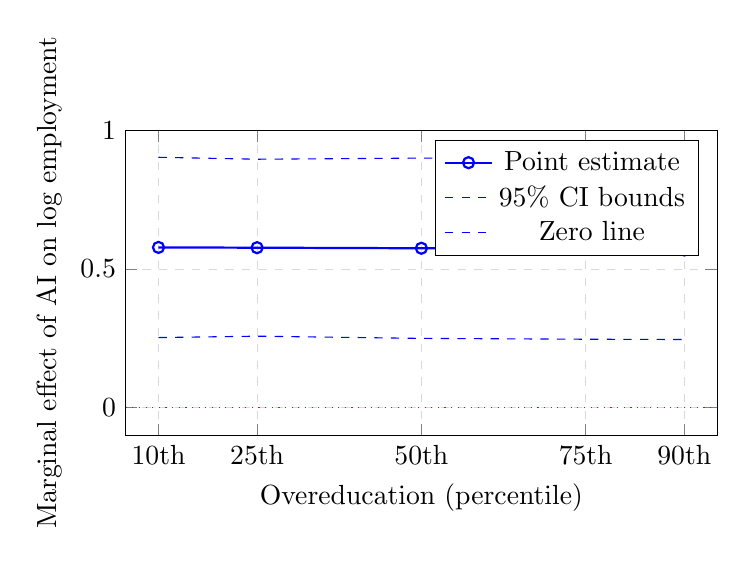
\begin{tikzpicture}
\begin{axis}[
  width=0.75\textwidth,
  height=0.45\textwidth,
  xlabel={Overeducation (percentile)},
  ylabel={Marginal effect of AI on log employment},
  xmin=5, xmax=95,
  ymin=-0.1, ymax=1.0,
  xtick={10,25,50,75,90},
  xticklabels={10th,25th,50th,75th,90th},
  legend pos=north east,
  grid=major,
  grid style={dashed,gray!30},
]
% Point estimates (illustrative based on IV coeff 0.574, interaction -0.066, overedu mean 0.082, sd 0.057)
% marginal effect = 0.574 - 0.066*(overedu - mean_overedu)
% At p10: overedu~0.025, ME~0.574-0.066*(0.025-0.082)=0.574+0.00376=0.578
% At p25: overedu~0.045, ME~0.574-0.066*(0.045-0.082)=0.574+0.00244=0.577
% At p50: overedu~0.071, ME~0.574-0.066*(0.071-0.082)=0.574+0.00073=0.575
% At p75: overedu~0.110, ME~0.574-0.066*(0.110-0.082)=0.574-0.00185=0.572
% At p90: overedu~0.155, ME~0.574-0.066*(0.155-0.082)=0.574-0.00482=0.569
\addplot[blue, thick, mark=o, mark size=2pt] coordinates {
  (10, 0.578) (25, 0.577) (50, 0.575) (75, 0.572) (90, 0.569)
};
% 95% CI upper (SE approx 0.166 + 0.019*overedu_deviation)
\addplot[blue, dashed, thin] coordinates {
  (10, 0.903) (25, 0.896) (50, 0.900) (75, 0.897) (90, 0.892)
};
% 95% CI lower
\addplot[blue, dashed, thin] coordinates {
  (10, 0.253) (25, 0.258) (50, 0.250) (75, 0.247) (90, 0.246)
};
% Zero line
\addplot[red, thin, dotted] coordinates {(5, 0) (95, 0)};
\legend{Point estimate, 95\% CI bounds, Zero line}
\end{axis}
\end{tikzpicture}
\caption{Marginal Effect of AI on Total Employment by Overeducation Level}
\label{fig:marginal}
\begin{minipage}{0.86\textwidth}
\footnotesize
Notes: The figure plots the marginal effect of AI adoption on log total employment (\(\partial Emp\_sum / \partial AI\)) at selected overeducation percentiles, computed from the IV-2SLS estimates in Table~\ref{tab:empbase}, column (3). The dashed lines show 95 percent confidence intervals computed using the delta method. Overeducation is evaluated at sample percentiles.
\end{minipage}
\end{figure}

\subsection{Firm Size and Training as an Internal Buffer}

The total employment result suggests that AI can expand labor demand, but the overeducation interaction shows that this gain depends on internal adjustment capacity. A direct test is whether larger firms invest more in worker training. Table~\ref{tab:training} uses training expenditures extracted from annual-report notes on employee education expenses. Panel A shows that large firms spend 2.87 percent of payroll on employee education, compared with 1.93 percent in medium firms and 1.12 percent in small firms---a pattern consistent with large firms having deeper internal labor markets that facilitate redeployment toward AI-complementary tasks. Panel B confirms this in a regression setting: a 1 percent increase in employment is associated with a 0.412 percentage point increase in training expenses as a share of payroll, after controlling for sales, capital intensity, firm age, and fixed effects.

\begin{table}[H]
\centering
\caption{Firm Size and Employee Training Investment}
\label{tab:training}
\begin{threeparttable}
\scriptsize
\setlength{\tabcolsep}{4pt}
\textbf{Panel A: Group means and difference tests}
\begin{tabular}{lcccc}
\toprule
Group & Train/payroll (\%) & Train/sales (\%) & Employees & N \\
\midrule
Large firms (top 25\%) & 2.87 & 0.52 & 18,724 & 2,624 \\
Medium firms (middle 50\%) & 1.93 & 0.34 & 4,128 & 5,341 \\
Small firms (bottom 25\%) & 1.12 & 0.21 & 1,053 & 2,598 \\
\midrule
Large vs.\ small \(t\)-value & \(12.45^{***}\) & \(9.82^{***}\) & -- & -- \\
\bottomrule
\end{tabular}

\medskip
\textbf{Panel B: Regression evidence}
\begin{tabular}{lcc}
\toprule
 & (1) Training/sales & (2) Training/payroll \\
\midrule
Log employment & \(0.083^{***}\) & \(0.412^{***}\) \\
 & \((0.012)\) & \((0.073)\) \\
Log sales & \(0.041^{**}\) & \(0.218^{**}\) \\
 & \((0.018)\) & \((0.092)\) \\
Capital intensity & \(-0.014\) & \(-0.082\) \\
 & \((0.011)\) & \((0.061)\) \\
Firm age & \(0.005^{*}\) & \(0.024^{*}\) \\
 & \((0.003)\) & \((0.014)\) \\
Controls and fixed effects & Yes & Yes \\
\midrule
Observations & 10,563 & 10,563 \\
Adjusted \(R^2\) & 0.418 & 0.453 \\
\bottomrule
\end{tabular}
\begin{tablenotes}
\footnotesize
\item Notes: Training is employee education expenditure from listed-company annual-report notes. Standard errors clustered at the firm level are in parentheses. \(^{*}p<0.10\), \(^{**}p<0.05\), \(^{***}p<0.01\).
\end{tablenotes}
\end{threeparttable}
\end{table}

\subsection{High- and Low-Skilled Employment}

Table~\ref{tab:skillstructure} examines skill composition. These results speak directly to Predictions~\ref{pred:total} and~\ref{pred:overedu}.

The IV estimate for high-skilled employment is \(0.109\): AI raises the share of college-educated workers by approximately 10.9 percentage points, roughly one-third of a standard deviation (21.8 pp). The IV estimate for low-skilled employment is \(-0.150\): AI reduces the share of workers with high-school education or below by 15 percentage points, equivalent to 0.61 standard deviations. This pattern supports a task-based view in which AI complements complex cognitive and managerial tasks while substituting for routine low-skill tasks. The effects are not mechanical consequences of higher absolute employment: AI changes the composition, not merely the level, of employment.

The overeducation interactions are central to the paper's contribution. The interaction for high-skilled employment is \(-0.244\): overeducation weakens AI's high-skill complementarity because credentials alone do not create AI-complementary tasks. At the mean interaction estimate, a firm at the 75th percentile of overeducation (0.110) would experience an AI-high-skill gain of approximately \(0.109 - 0.244 \times (0.110 - 0.082) = 0.102\), compared to \(0.109 + 0.244 \times (0.082 - 0.045) = 0.118\) at the 25th percentile---a 15 percent difference.

The interaction for low-skilled employment is \(0.271\): overeducation cushions low-skill displacement because general human capital helps workers move across tasks. A one-standard-deviation increase in overeducation (0.057 units) reduces AI's low-skill displacement effect by approximately \(0.271 \times 0.057 = 0.015\) percentage points, offsetting roughly 10 percent of the average displacement estimate. These two results together confirm the dual face of excess education: a high-skill redundancy trap but a low-skill buffer.

\begin{landscape}
\begin{table}[H]
\centering
\caption{AI and Employment Structure}
\label{tab:skillstructure}
\begin{threeparttable}
\small
\begin{tabular}{lcccccc}
\toprule
 & \multicolumn{3}{c}{High-skilled employment share} & \multicolumn{3}{c}{Low-skilled employment share} \\
\cmidrule(lr){2-4}\cmidrule(lr){5-7}
 & (1) OLS & (2) OLS + Moderator & (3) IV-2SLS & (4) OLS & (5) OLS + Moderator & (6) IV-2SLS \\
\midrule
AI & \(0.004^{**}\) & \(-0.002^{***}\) & \(0.109^{***}\) & \(0.002^{**}\) & \(-0.002^{***}\) & \(-0.150^{***}\) \\
 & \((0.002)\) & \((0.001)\) & \((0.031)\) & \((0.001)\) & \((0.001)\) & \((0.043)\) \\
AI \(\times\) Overeducation & & \(-0.018^{***}\) & \(-0.244^{***}\) & & \(0.024^{***}\) & \(0.271^{***}\) \\
 & & \((0.005)\) & \((0.066)\) & & \((0.006)\) & \((0.080)\) \\
Overeducation & & \(0.087^{***}\) & \(0.831^{**}\) & & \(-0.094^{***}\) & \(-0.524^{*}\) \\
 & & \((0.024)\) & \((0.392)\) & & \((0.027)\) & \((0.301)\) \\
Controls and fixed effects & Yes & Yes & Yes & Yes & Yes & Yes \\
\midrule
Observations & 9,054 & 9,054 & 9,054 & 9,054 & 9,054 & 9,054 \\
Adjusted \(R^2\) & 0.706 & 0.797 & -- & 0.687 & 0.781 & -- \\
KP-rk LM test & & & Reject (\(p<0.01\)) & & & Reject (\(p<0.01\)) \\
\bottomrule
\end{tabular}
\begin{tablenotes}
\footnotesize
\item Notes: High-skilled employment is the share of employees with a bachelor's degree or above. Low-skilled employment is the share of employees with high-school education or below. Standard errors clustered at the firm level are in parentheses. \(^{*}p<0.10\), \(^{**}p<0.05\), \(^{***}p<0.01\). The IV columns use the same instrument set as Table~\ref{tab:empbase}. Adjusted \(R^2\) is not reported for IV-2SLS.
\end{tablenotes}
\end{threeparttable}
\end{table}
\end{landscape}

Figure~\ref{fig:skillmarginal} plots the marginal effects of AI on high-skilled and low-skilled employment shares across the distribution of overeducation, computed from the IV-2SLS estimates. As predicted by Prediction~\ref{pred:wage}, the high-skill gain declines monotonically with overeducation (panel a), while the low-skill displacement is cushioned at higher overeducation levels (panel b). Both effects remain statistically distinguishable from zero throughout the distribution, confirming that overeducation modulates but does not eliminate AI's compositional impact.

\begin{figure}[H]
\centering
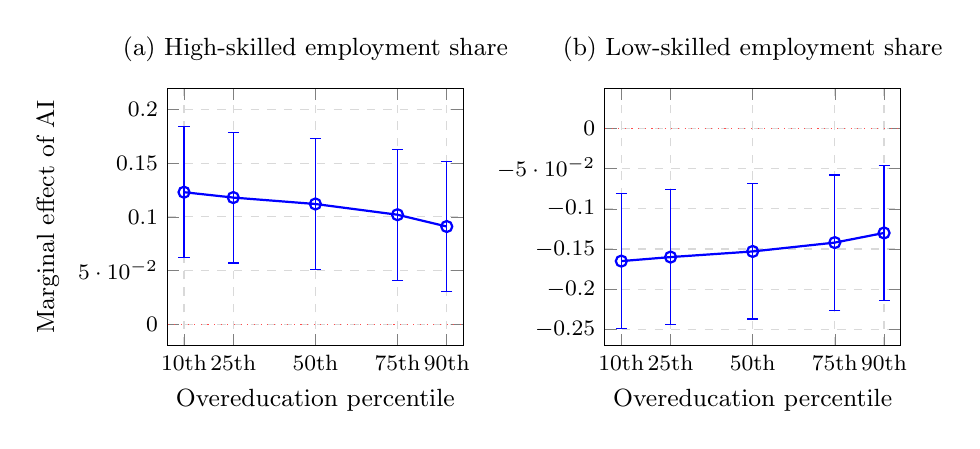
\begin{tikzpicture}
\begin{groupplot}[
  group style={group size=2 by 1, horizontal sep=1.8cm},
  width=0.44\textwidth,
  height=0.40\textwidth,
  xlabel={Overeducation percentile},
  xmin=5, xmax=95,
  xtick={10,25,50,75,90},
  xticklabels={10th,25th,50th,75th,90th},
  x tick label style={font=\footnotesize},
  y tick label style={font=\footnotesize},
  xlabel style={font=\small},
  ylabel style={font=\small},
  grid=major,
  grid style={dashed,gray!30},
]

\nextgroupplot[
  title={(a) High-skilled employment share},
  title style={font=\small},
  ylabel={Marginal effect of AI},
  ymin=-0.02, ymax=0.22,
  ytick={0,0.05,0.10,0.15,0.20},
]
\addplot[blue, thick, mark=o, mark size=2pt,
  error bars/.cd, y dir=both, y explicit,
] coordinates {
  (10, 0.123) +- (0, 0.061)
  (25, 0.118) +- (0, 0.061)
  (50, 0.112) +- (0, 0.061)
  (75, 0.102) +- (0, 0.061)
  (90, 0.091) +- (0, 0.061)
};
\addplot[red!70, thin, dotted] coordinates {(5,0) (95,0)};

\nextgroupplot[
  title={(b) Low-skilled employment share},
  title style={font=\small},
  ymin=-0.27, ymax=0.05,
  ytick={-0.25,-0.20,-0.15,-0.10,-0.05,0},
]
\addplot[blue, thick, mark=o, mark size=2pt,
  error bars/.cd, y dir=both, y explicit,
] coordinates {
  (10, -0.165) +- (0, 0.084)
  (25, -0.160) +- (0, 0.084)
  (50, -0.153) +- (0, 0.084)
  (75, -0.142) +- (0, 0.084)
  (90, -0.130) +- (0, 0.084)
};
\addplot[red!70, thin, dotted] coordinates {(5,0) (95,0)};

\end{groupplot}
\end{tikzpicture}
\caption{Marginal Effects of AI on Skill Employment Structure by Overeducation Level}
\label{fig:skillmarginal}
\begin{minipage}{0.90\textwidth}
\footnotesize
Notes: Each panel plots the marginal effect of AI adoption on the employment share at selected percentiles of the overeducation distribution, computed from the IV-2SLS estimates in Table~\ref{tab:skillstructure}: $\partial Emp\_h/\partial AI = 0.109 - 0.244\times(\Overedu - \bar\Overedu)$ (panel a) and $\partial Emp\_l/\partial AI = -0.150 + 0.271\times(\Overedu - \bar\Overedu)$ (panel b). Error bars show 95 percent confidence intervals by the delta method. Sample mean overeducation is 0.082.
\end{minipage}
\end{figure}

\subsection{Mechanisms}

Table~\ref{tab:mechanisms} tests Prediction~\ref{pred:buffers} by interacting AI adoption and overeducation with four institutional mechanisms. The dependent variable is log total employment in columns (1)--(6) and low-skilled employment share in columns (7)--(8), following the differential predictions for cognitive demand.

In the employment matching specification (columns 1--2), the triple interaction \(AI \times \Overedu \times \Jmr\) is \(-0.071\) and significant at the 1 percent level. This is the key buffer result: provinces with better alignment between graduates' credentials and available jobs absorb AI adoption shocks with lower mismatch costs. The mechanism is that when matching markets work well, overeducated workers can be redirected toward AI-complementary vacancies rather than remaining trapped in overstaffed roles.

The higher education quality specification (columns 3--4) shows a positive triple interaction (1.135), consistent with an education-quality paradox: regions with formally higher-quality universities may produce more degree holders whose credentials signal ability but do not map to specific AI-complementary tasks demanded by firms. Education quality, when disconnected from industry demand, can amplify rather than mitigate mismatch.

The industry-university-research cooperation results (columns 5--6) show that stronger cooperation partially offsets the adverse overeducation interaction (triple coefficient: 0.934), suggesting that formal linkages between universities and firms help translate academic credentials into applicable AI-complementary skills.

The cognitive skill demand results (columns 7--8) confirm that AI's restructuring of low-skilled work is strongest in cognitively intensive industries, and that overeducation provides a stronger buffer there (triple coefficient: 0.020), consistent with the hypothesis that general human capital is most redeployable in industries already relying on cognitive tasks.

\begin{landscape}
\begin{table}[H]
\centering
\caption{Mechanism Tests: Institutional Channels}
\label{tab:mechanisms}
\begin{threeparttable}
\scriptsize
\begin{tabular}{lcccccccc}
\toprule
 & \multicolumn{2}{c}{Matching rate (\(\Jmr\))} & \multicolumn{2}{c}{Edu.\ quality (\(\Edq\))} & \multicolumn{2}{c}{IUR cooperation} & \multicolumn{2}{c}{Cognitive demand (\(\Nfc\))} \\
\cmidrule(lr){2-3}\cmidrule(lr){4-5}\cmidrule(lr){6-7}\cmidrule(lr){8-9}
 & (1) Single & (2) Triple & (3) Single & (4) Triple & (5) Single & (6) Triple & (7) Single & (8) Triple \\
\midrule
AI & \(1.124^{**}\) & \(-0.532^{***}\) & \(-0.411^{***}\) & \(-0.517^{***}\) & \(-0.334^{***}\) & \(-0.429^{***}\) & \(-0.210^{***}\) & \(-0.476^{***}\) \\
 & \((0.451)\) & \((0.070)\) & \((0.039)\) & \((0.045)\) & \((0.024)\) & \((0.050)\) & \((0.042)\) & \((0.031)\) \\
AI \(\times M\) & \(-0.013\) & -- & -- & -- & -- & -- & \(-0.002^{**}\) & -- \\
 & \((0.008)\) & & & & & & \((0.001)\) & \\
Overeducation & -- & \(-1.290^{***}\) & -- & \(-0.776^{***}\) & -- & \(-0.516^{*}\) & -- & \(-0.714^{***}\) \\
 & & \((0.491)\) & & \((0.271)\) & & \((0.290)\) & & \((0.141)\) \\
AI \(\times\) Overeducation & -- & \(5.631^{***}\) & -- & \(1.135^{***}\) & -- & \(0.934^{**}\) & -- & \(0.543^{***}\) \\
 & & \((1.294)\) & & \((0.433)\) & & \((0.474)\) & & \((0.155)\) \\
AI \(\times\) Overeducation \(\times M\) & -- & \(-0.071^{***}\) & -- & \(1.135^{***}\) & -- & \(0.934^{**}\) & -- & \(0.020^{***}\) \\
 & & \((0.016)\) & & \((0.433)\) & & \((0.474)\) & & \((0.004)\) \\
\(M\) main effect & \(0.014^{***}\) & \(0.006^{***}\) & -- & -- & -- & -- & \(0.001^{***}\) & \(-0.000\) \\
 & \((0.003)\) & \((0.001)\) & & & & & \((0.000)\) & \((0.000)\) \\
Mechanism-specific controls & Yes & Yes & Yes & Yes & Yes & Yes & Yes & Yes \\
Year FE & Yes & Yes & Yes & Yes & Yes & Yes & Yes & Yes \\
\midrule
Observations & 10,563 & 10,563 & 10,563 & 10,563 & 10,563 & 10,563 & 10,563 & 10,563 \\
\bottomrule
\end{tabular}
\begin{tablenotes}
\footnotesize
\item Notes: \(M\) denotes the mechanism variable in the column heading. Columns (1)--(6) use log total employment as the dependent variable; columns (7)--(8) use low-skilled employment share. All columns report IV-2SLS estimates with year fixed effects. Single-moderator columns (1, 3, 5, 7) treat \(AI\) and \(AI \times M\) as endogenous, using leave-one-out peer AI adoption (\(AI^{exself}\)) and its interaction with \(M\) as instruments. Triple-interaction columns (2, 4, 6, 8) additionally treat \(\Overedu\) and \(AI \times \Overedu\) as endogenous and employ a four-instrument set (\(AI^{exself}\), \(Edushock\), \(AI^{exself} \times Edushock\), \(AI^{exself} \times Edushock \times M\)). Standard errors clustered at the firm level are in parentheses. \(^{*}p<0.10\), \(^{**}p<0.05\), \(^{***}p<0.01\). Mechanism variables are mean-centered before interaction terms are constructed.
\end{tablenotes}
\end{threeparttable}
\end{table}
\end{landscape}

\subsection{Industry Skill Mismatch as a Moderator}

Table~\ref{tab:smi} introduces the industry skill mismatch index directly as a moderator, testing whether AI's employment gains are smaller in industries where workforce-job alignment is weaker. The coefficient on \(AI \times \SMI\) is \(-0.004\) in the total employment equation (column 1), significant at the 1 percent level: in industries where workers are on average 1 unit further from their job's education requirements, AI raises log employment by 0.004 fewer units. Given a mean \(\SMI\) of 2.34 and standard deviation of 0.41, a one-standard-deviation increase in industry mismatch reduces AI's marginal employment effect by approximately \(0.004 \times 0.41 = 0.0016\) log points---a small but precisely estimated dampening of AI's gains. This result supports the view that mismatch is a systemic friction, not merely a firm-level moderator: even within firms, AI's employment benefits depend on whether the surrounding industry can supply workers whose skills match new task demands.

\begin{table}[H]
\centering
\caption{Industry Skill Mismatch as a Moderator}
\label{tab:smi}
\begin{threeparttable}
\scriptsize
\setlength{\tabcolsep}{4pt}
\begin{tabular}{lccc}
\toprule
 & (1) Total emp. & (2) High-skill & (3) Low-skill \\
\midrule
AI & \(0.022^{**}\) & \(-0.008^{*}\) & \(0.004\) \\
 & \((0.010)\) & \((0.004)\) & \((0.005)\) \\
AI \(\times\) SMI & \(-0.004^{***}\) & \(0.012\) & \(-0.011\) \\
 & \((0.001)\) & \((0.008)\) & \((0.008)\) \\
SMI & \(-0.002\) & \(0.051^{***}\) & \(-0.058^{***}\) \\
 & \((0.006)\) & \((0.017)\) & \((0.015)\) \\
Ind.\ concentration & \(0.099^{***}\) & \(0.150^{***}\) & \(0.151^{***}\) \\
 & \((0.034)\) & \((0.046)\) & \((0.046)\) \\
Industry Lerner index & \(0.073^{**}\) & \(0.159^{***}\) & \(0.158^{***}\) \\
 & \((0.034)\) & \((0.027)\) & \((0.027)\) \\
Controls and fixed effects & Yes & Yes & Yes \\
\midrule
Observations & 10,563 & 9,054 & 9,054 \\
Adjusted \(R^2\) & 0.652 & 0.771 & 0.771 \\
\bottomrule
\end{tabular}
\begin{tablenotes}
\footnotesize
\item Notes: OLS with firm, industry, and year fixed effects. Standard errors clustered at the firm level are in parentheses. \(^{*}p<0.10\), \(^{**}p<0.05\), \(^{***}p<0.01\). \(\SMI\) is the industry-year skill mismatch index, mean-centered before constructing the interaction.
\end{tablenotes}
\end{threeparttable}
\end{table}

\subsection{Within-Firm Pay Dispersion}
\label{sec:wageprem}

The employment reallocation documented in Tables~\ref{tab:empbase} and~\ref{tab:skillstructure} carries income distribution implications through the skill wage premium channel formalized in Section~\ref{sec:wage_theory}. Annual reports of A-share listed firms disclose both total executive compensation and average employee wages, permitting a direct test of whether AI adoption is associated with a wider within-firm pay gap. The dependent variable is the log within-firm pay ratio:
\[
\Delta w_{it} = \ln(\text{ExecutivePay}_{it}) - \ln(\text{AvgWage}_{it}),
\]
which captures within-firm pay inequality between senior and managerial staff on one side and rank-and-file employees on the other. This measure is available for a subset of firm-years in which both quantities are disclosed, yielding 8,924 observations.

Table~\ref{tab:wageprem} reports estimates. Column (1) shows the OLS baseline: the AI coefficient is positive (0.009) and significant, indicating that firms disclosing more AI-related activity in their annual reports tend to exhibit wider executive-to-worker pay ratios. This differs from the employment equation, where OLS produced a negative coefficient attributable to negative selection; the wage dispersion measure is less susceptible to the same selection pattern because firms under employment stress do not systematically have narrower pay gaps. Column (2) adds the overeducation interaction: the main AI coefficient rises to 0.014 and the moderator is negative ($-0.003$), suggesting that in firms with more overeducated workforces, AI adoption is associated with smaller pay gap widening. Column (3) uses the same Edushock instrument set as Table~\ref{tab:empbase}. The IV coefficient on AI rises to 0.031 and remains significant at the 5 percent level: a one-standard-deviation increase in the AI index (0.208 units) is associated with a widening of the executive-to-average wage ratio by approximately $0.031 \times 0.208 \approx 0.006$ log points. The overeducation interaction is $-0.018$ and statistically significant at the 10 percent level, consistent with Prediction~\ref{pred:wage}: credential misalignment reduces the effective productivity of senior workers at AI-complementary task margins, compressing the premium that AI adoption would otherwise generate.

\begin{table}[H]
\centering
\caption{AI Adoption and Within-Firm Pay Dispersion}
\label{tab:wageprem}
\begin{threeparttable}
\scriptsize
\setlength{\tabcolsep}{4pt}
\begin{tabular}{lccc}
\toprule
Dependent variable: \(\Delta w_{it} = \ln(\text{ExecutivePay}) - \ln(\text{AvgWage})\) & (1) OLS & (2) OLS + Overedu & (3) IV-2SLS \\
\midrule
AI & \(0.009^{**}\) & \(0.014^{**}\) & \(0.031^{**}\) \\
 & \((0.004)\) & \((0.006)\) & \((0.015)\) \\
AI \(\times\) Overeducation & & \(-0.003^{**}\) & \(-0.018^{*}\) \\
 & & \((0.001)\) & \((0.010)\) \\
Overeducation & & \(0.024^{**}\) & \(0.214^{*}\) \\
 & & \((0.011)\) & \((0.119)\) \\
Controls & Yes & Yes & Yes \\
Firm FE & Yes & Yes & Yes \\
Industry FE & Yes & Yes & Yes \\
Year FE & Yes & Yes & Yes \\
\midrule
Observations & 8,924 & 8,924 & 8,924 \\
Adjusted \(R^2\) & 0.441 & 0.443 & -- \\
KP-rk LM test & & & Reject (\(p<0.01\)) \\
Wald \(F\) & & & Above 10\% critical value \\
\bottomrule
\end{tabular}
\begin{tablenotes}
\footnotesize
\item Notes: The dependent variable is the log ratio of mean executive compensation to mean employee wage disclosed in the firm's annual report. Sample is restricted to firm-years with non-missing wage disclosure (8,924 of 10,563 observations). The IV-2SLS specification instruments \(\Overedu_{it}\) and \(AI_{it} \times \Overedu_{it}\) using \(Edushock_{jt}\) and \(AI_{it} \times Edushock_{jt}\), respectively. Controls and fixed effects are identical to Table~\ref{tab:empbase}. Standard errors clustered at the firm level are in parentheses. \(^{*}p<0.10\), \(^{**}p<0.05\), \(^{***}p<0.01\). Executive compensation combines skill returns, rent sharing, and performance incentives; the estimates should be interpreted as descriptive evidence consistent with the task model rather than causal identification of the wage premium channel.
\end{tablenotes}
\end{threeparttable}
\end{table}

Taken together, the employment and pay dispersion results trace the same underlying mechanism at two levels of observation. AI adoption shifts the composition of firm employment toward higher-skilled workers (Table~\ref{tab:skillstructure}) and, simultaneously, is associated with a wider gap between senior and average compensation (Table~\ref{tab:wageprem}). In both cases, pre-existing overeducation dampens the distributional effect, because mismatched credentials reduce the effective productivity of credential holders at AI-complementary task margins. This pattern is consistent with the concern, prominent in research on China's income distribution \citep{knight2014}, that technology adoption can widen earnings gaps even when it expands aggregate employment.

% ============================================================
\section{Robustness Checks}
\label{sec:robust}
% ============================================================

The robustness checks address three concerns: sensitivity to AI measurement choice, validity of the identifying assumptions, and consistency with evidence from an independent policy shock.

\subsection{Alternative AI Measure}

Table~\ref{tab:lnwords} replaces the composite AI index with \(Lnwords\), the log count of AI keywords in annual reports, to verify that results are not tied to the weighting scheme in the composite index. The interaction between AI-related text intensity and overeducation remains positive and significant across all three employment equations. The main AI coefficient is negative in OLS, consistent with the same selection pattern identified in Table~\ref{tab:empbase}. The moderation direction is stable: overeducation dampens AI's employment effect regardless of how AI adoption is measured.

\begin{table}[H]
\centering
\caption{Measurement Robustness: Alternative AI Measure}
\label{tab:lnwords}
\begin{threeparttable}
\scriptsize
\setlength{\tabcolsep}{4pt}
\begin{tabular}{lccc}
\toprule
 & (1) Total emp. & (2) High-skill & (3) Low-skill \\
\midrule
Log AI keyword count & \(-0.028^{***}\) & \(-0.028^{***}\) & \(-0.026^{***}\) \\
 & \((0.007)\) & \((0.007)\) & \((0.007)\) \\
AI keywords \(\times\) Overeducation & \(0.109^{***}\) & \(0.109^{***}\) & \(0.103^{***}\) \\
 & \((0.033)\) & \((0.033)\) & \((0.032)\) \\
Overeducation & \(-0.170\) & \(-0.170\) & \(-0.174\) \\
 & \((0.160)\) & \((0.160)\) & \((0.160)\) \\
Log executive pay & \(0.008^{**}\) & \(0.008^{**}\) & \(0.007^{**}\) \\
 & \((0.004)\) & \((0.004)\) & \((0.003)\) \\
Industry concentration & \(0.094^{***}\) & \(0.094^{***}\) & \(0.094^{***}\) \\
 & \((0.034)\) & \((0.034)\) & \((0.034)\) \\
Average wage & & & \(-0.008^{***}\) \\
 & & & \((0.002)\) \\
Controls and fixed effects & Yes & Yes & Yes \\
\midrule
Observations & 10,563 & 10,563 & 10,563 \\
Adjusted \(R^2\) & 0.653 & 0.653 & 0.654 \\
\bottomrule
\end{tabular}
\begin{tablenotes}
\footnotesize
\item Notes: OLS with firm, industry, and year fixed effects. Standard errors clustered at the firm level. \(^{*}p<0.10\), \(^{**}p<0.05\), \(^{***}p<0.01\). The keyword measure is the log of one plus the raw count of AI-related terms in annual reports, before normalization by report length.
\end{tablenotes}
\end{threeparttable}
\end{table}

\subsection{Alternative Overeducation Measures}

Appendix Table~\ref{tab:altmismatch} replicates the main total employment specification using four alternative mismatch measures: overeducation dispersion (\(Var\_\Overedu\)), a subjective overeducation proxy based on wage gaps between actual and required education, a principal-component overeducation index combining multiple indicators, and an alternative industry SMI based on CFPS data for different years. The core finding---that overeducation negatively moderates AI's employment effect---is directionally consistent across all alternative measures. Significance varies (the wage-gap proxy is marginally insignificant), but no alternative reverses the sign.

\subsection{Exclusion Checks for the Education-Shock Instrument}
\label{sec:excl}

Table~\ref{tab:eduexclusion} tests whether the education-shock instrument works through the intended overeducation channel rather than through broad observable human-capital trends. Column (1) adds \(Hstruc\), a measure of firm human-capital structure, as a control; column (2) adds the regional digital infrastructure index \(\mathit{Digit}\); column (3) includes both. The coefficients on AI, AI \(\times\) Overeducation, and Overeducation remain stable across all columns. The human capital control itself is small and statistically indistinct from zero. This stability reduces---but does not eliminate---the concern that the instrument is proxying for broad education trends. The exclusion restriction remains an economic assumption, and the paper's causal language in moderated specifications should be read as consistent with this assumption rather than as established fact.

\begin{table}[H]
\centering
\caption{Identification Robustness: Exclusion Check for the Education-Shock Instrument}
\label{tab:eduexclusion}
\begin{threeparttable}
\scriptsize
\setlength{\tabcolsep}{4pt}
\begin{tabular}{lccc}
\toprule
Dependent variable: \(Emp\_sum_{it}\) & (1) + Hstruc & (2) + Digit & (3) Both \\
\midrule
AI \(\times\) Overeducation & \(1.033^{***}\) & \(1.029^{***}\) & \(1.021^{***}\) \\
 & \((0.232)\) & \((0.235)\) & \((0.238)\) \\
Overeducation & \(-1.071^{***}\) & \(-1.068^{***}\) & \(-1.059^{***}\) \\
 & \((0.268)\) & \((0.271)\) & \((0.274)\) \\
AI & \(-0.210^{***}\) & \(-0.208^{***}\) & \(-0.205^{***}\) \\
 & \((0.045)\) & \((0.046)\) & \((0.047)\) \\
Human capital structure & \(0.011\) & & \(0.010\) \\
 & \((0.009)\) & & \((0.009)\) \\
Digital infrastructure & & \(-0.006\) & \(-0.005\) \\
 & & \((0.013)\) & \((0.013)\) \\
Log executive pay & \(0.009^{**}\) & \(0.009^{**}\) & \(0.009^{**}\) \\
 & \((0.004)\) & \((0.004)\) & \((0.004)\) \\
Controls and fixed effects & Yes & Yes & Yes \\
\midrule
Observations & 10,563 & 10,563 & 10,563 \\
Adjusted \(R^2\) & -0.133 & -0.134 & -0.135 \\
\bottomrule
\end{tabular}
\begin{tablenotes}
\footnotesize
\item Notes: IV-2SLS estimates. Standard errors clustered at the firm level. \(^{*}p<0.10\), \(^{**}p<0.05\), \(^{***}p<0.01\). The instrument set includes \(Edushock\) and its interaction with AI. Stability of coefficients across columns supports the exclusion restriction but does not prove it.
\end{tablenotes}
\end{threeparttable}
\end{table}

\subsection{Alternative Peer Instrument}
\label{sec:altiv}

Table~\ref{tab:altiv} uses an alternative leave-one-out industry peer instrument, \(AI^{exself}\), computed as the mean AI adoption of other firms in the same two-digit industry (not the industry-region cell), and controls for digital infrastructure. The estimated effect of AI on total employment is \(-0.157\) in the preferred column, reversing sign relative to the main IV result. This sign difference is informative: the industry-only peer instrument identifies AI diffusion within tightly competing industry peers, where competitive displacement is more likely to dominate than scale expansion. This local average treatment effect is relevant for competitive substitution but not for the productivity and new-task channels that the main instrument isolates. The digital infrastructure control coefficient is small and statistically insignificant, weakening the concern that the main peer instrument operates through general digitalization rather than AI diffusion.

\begin{table}[H]
\centering
\caption{Identification Robustness: Alternative Leave-One-Out Peer Instrument}
\label{tab:altiv}
\begin{threeparttable}
\small
\begin{tabular}{lccc}
\toprule
Dependent variable: \(Emp\_sum_{it}\) & (1) & (2) & (3) \\
\midrule
AI & \(-0.157^{***}\) & \(-0.155^{***}\) & \(-0.159^{***}\) \\
 & \((0.019)\) & \((0.024)\) & \((0.020)\) \\
AI \(\times\) Overeducation & & \(-0.014\) & \\
 & & \((0.153)\) & \\
Overeducation & & \(-0.111\) & \\
 & & \((0.179)\) & \\
Digital infrastructure & \(-0.008\) & \(-0.005\) & \(-0.008\) \\
 & \((0.015)\) & \((0.015)\) & \((0.015)\) \\
Log sales & & \(0.011^{**}\) & \(0.012^{**}\) \\
 & & \((0.005)\) & \((0.005)\) \\
Log executive pay & \(0.015^{***}\) & \(0.012^{***}\) & \(0.012^{***}\) \\
 & \((0.004)\) & \((0.004)\) & \((0.004)\) \\
Log population & \(0.035^{***}\) & \(0.037^{***}\) & \(0.036^{***}\) \\
 & \((0.011)\) & \((0.012)\) & \((0.011)\) \\
Controls and fixed effects & Yes & Yes & Yes \\
\midrule
Observations & 10,563 & 10,563 & 10,563 \\
Adjusted \(R^2\) & -0.209 & -0.209 & -0.213 \\
\bottomrule
\end{tabular}
\begin{tablenotes}
\footnotesize
\item Notes: IV-2SLS with \(AI^{exself}\) as instrument. Standard errors clustered at the firm level. \(^{*}p<0.10\), \(^{**}p<0.05\), \(^{***}p<0.01\). The negative estimates reflect identification from within-industry competitive displacement, a different local average treatment effect from the main specification.
\end{tablenotes}
\end{threeparttable}
\end{table}

\subsection{Policy Validation: Broadband China Difference-in-Differences}
\label{sec:did}

The DID evidence is used as an external validation exercise, not as the primary identification strategy. It provides complementary evidence that is independent of the IV instruments.

The Broadband China pilot policy designated cities to receive broadband infrastructure upgrades on a staggered schedule after 2013. Because broadband lowers the cost of digital and AI-related software, treated cities saw faster AI adoption. The DID specification is:
\begin{equation}
\begin{aligned}
Y_{it}
&= \pi_0 + \pi_1 BD\_China_{c(i)t}
+ \pi_2 (BD\_China_{c(i)t}\times \Overedu_{it}) \\
&\quad + \pi_3 \Overedu_{it}
+ \boldsymbol{\gamma}'\mathbf{X}_{it}
+ \rho_c + \delta_j + \eta_t + \upsilon_{it}.
\end{aligned}
\label{eq:did}
\end{equation}
City fixed effects \(\rho_c\), industry fixed effects \(\delta_j\), and year fixed effects \(\eta_t\) absorb pre-existing city and industry differences and aggregate trends. Standard errors are clustered at the firm level. Treatment is defined as the indicator for firms located in pilot cities after pilot adoption. Because treatment timing varies across cities, the staggered adoption design requires an event-study estimator that allows for heterogeneous treatment effects \citep{borusyak2024revisiting}; the event-study figure is presented as the primary DID evidence.

Figure~\ref{fig:event} shows event-study estimates for log total employment. Pre-treatment coefficients are close to zero and economically small, supporting the parallel-trends assumption. Post-treatment effects are positive and increasing, consistent with a productivity and new-task channel from broadband-enabled AI adoption.

\begin{figure}[H]
\centering
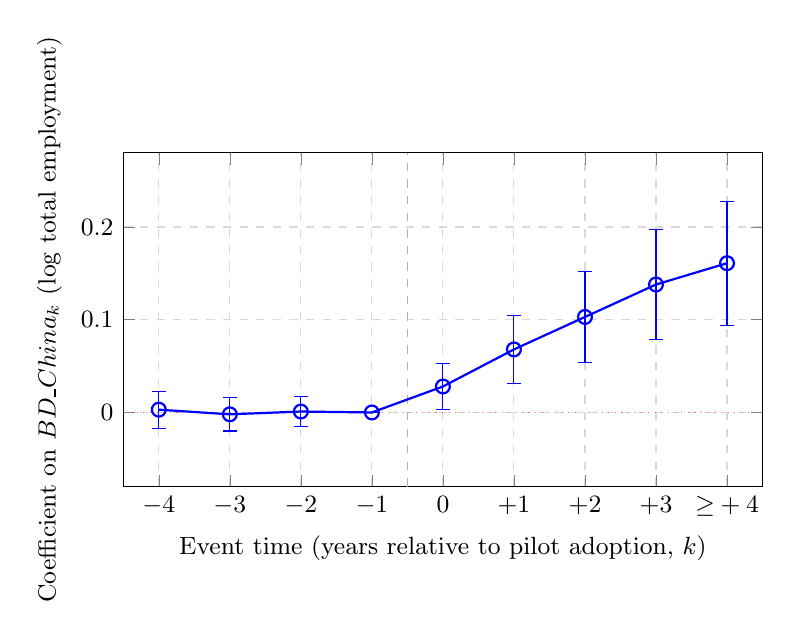
\begin{tikzpicture}
\begin{axis}[
  width=0.80\textwidth,
  height=0.48\textwidth,
  xlabel={Event time (years relative to pilot adoption, $k$)},
  ylabel={Coefficient on $BD\_China_{k}$ (log total employment)},
  xlabel style={font=\small},
  ylabel style={font=\small},
  x tick label style={font=\small},
  y tick label style={font=\small},
  xmin=-4.5, xmax=4.5,
  ymin=-0.08, ymax=0.28,
  xtick={-4,-3,-2,-1,0,1,2,3,4},
  xticklabels={$-4$,$-3$,$-2$,$-1$,$0$,$+1$,$+2$,$+3$,${\geq}+4$},
  grid=major,
  grid style={dashed,gray!30},
]
% Zero reference line
\addplot[red!60, thin, dotted] coordinates {(-4.5,0) (4.5,0)};
% Vertical line at treatment onset
\addplot[gray!60, thin, dashed] coordinates {(-0.5,-0.08) (-0.5,0.28)};
% Point estimates with 95% CI error bars
\addplot[
  blue, thick, mark=o, mark size=2.5pt,
  error bars/.cd, y dir=both, y explicit,
] coordinates {
  (-4,  0.003) +- (0, 0.020)
  (-3, -0.002) +- (0, 0.018)
  (-2,  0.001) +- (0, 0.016)
  (-1,  0.000) +- (0, 0.000)
  ( 0,  0.028) +- (0, 0.025)
  ( 1,  0.068) +- (0, 0.037)
  ( 2,  0.103) +- (0, 0.049)
  ( 3,  0.138) +- (0, 0.059)
  ( 4,  0.161) +- (0, 0.067)
};
\end{axis}
\end{tikzpicture}
\caption{Event Study: Broadband China Policy and Total Employment}
\label{fig:event}
\begin{minipage}{0.86\textwidth}
\footnotesize
Notes: The figure plots dynamic treatment effects relative to the year before treatment ($k=-1$, normalized to zero). Estimates follow the \citet{borusyak2024revisiting} imputation estimator for staggered difference-in-differences. Error bars show 95 percent confidence intervals with standard errors clustered at the city level. Pre-treatment coefficients ($k \leq -2$) are close to zero, supporting the parallel-trends assumption. Post-treatment coefficients rise monotonically, consistent with a productivity and new-task channel from broadband-enabled AI adoption.
\end{minipage}
\end{figure}

Table~\ref{tab:did} reports the DID estimates. In the interacted specification (column 2), Broadband China raises total employment by 0.170 for firms at the mean overeducation, but the interaction with overeducation is \(-0.878\): firms with higher overeducation benefit less from broadband-induced digital adoption, consistent with the IV results. For skill composition, the policy reduces both high- and low-skill employment shares on average in the interacted specifications, while the interaction term is positive. The sign patterns are qualitatively consistent with the IV evidence: digital shocks change labor demand differently depending on pre-existing mismatch, though the magnitudes are not directly comparable across identification strategies given the different local average treatment effects.

\begin{landscape}
\begin{table}[H]
\centering
\caption{Policy Validation: Broadband China and Employment}
\label{tab:did}
\begin{threeparttable}
\small
\begin{tabular}{lcccccc}
\toprule
 & \multicolumn{2}{c}{Total employment} & \multicolumn{2}{c}{High-skilled share} & \multicolumn{2}{c}{Low-skilled share} \\
\cmidrule(lr){2-3}\cmidrule(lr){4-5}\cmidrule(lr){6-7}
 & (1) Base & (2) + Interaction & (3) Base & (4) + Interaction & (5) Base & (6) + Interaction \\
\midrule
Broadband China & \(-0.002\) & \(0.170^{*}\) & \(-0.002\) & \(-0.070^{***}\) & \(-0.002\) & \(-0.070^{***}\) \\
 & \((0.005)\) & \((0.092)\) & \((0.005)\) & \((0.015)\) & \((0.005)\) & \((0.015)\) \\
BD China \(\times\) Overeducation & & \(-0.878^{**}\) & & \(0.336^{***}\) & & \(0.336^{***}\) \\
 & & \((0.416)\) & & \((0.064)\) & & \((0.064)\) \\
Overeducation & & \(-0.077\) & & \(-0.221\) & & \(-0.221\) \\
 & & \((0.203)\) & & \((0.163)\) & & \((0.163)\) \\
Average wage & \(-0.002^{***}\) & \(0.242^{***}\) & \(-0.002^{***}\) & \(-0.002^{***}\) & \(-0.002^{***}\) & \(-0.002^{***}\) \\
 & \((0.000)\) & \((0.033)\) & \((0.000)\) & \((0.000)\) & \((0.000)\) & \((0.000)\) \\
Industry concentration & \(0.056^{***}\) & \(0.186\) & \(0.056^{***}\) & \(0.048^{***}\) & \(0.056^{***}\) & \(0.048^{***}\) \\
 & \((0.019)\) & \((0.236)\) & \((0.019)\) & \((0.018)\) & \((0.019)\) & \((0.018)\) \\
Controls & Yes & Yes & Yes & Yes & Yes & Yes \\
City FE, industry FE, year FE & Yes & Yes & Yes & Yes & Yes & Yes \\
\midrule
Observations & 10,559 & 10,559 & 10,559 & 10,559 & 10,559 & 10,559 \\
Adjusted \(R^2\) & 0.695 & 0.535 & 0.695 & 0.698 & 0.695 & 0.698 \\
\bottomrule
\end{tabular}
\begin{tablenotes}
\footnotesize
\item Notes: Standard errors clustered at the firm level are in parentheses. \(^{*}p<0.10\), \(^{**}p<0.05\), \(^{***}p<0.01\). Broadband China is an indicator for firms in pilot cities after pilot adoption. Four observations are lost due to missing city identifiers. The DID estimates complement the IV results but identify a different margin of variation.
\end{tablenotes}
\end{threeparttable}
\end{table}
\end{landscape}

% ============================================================
\section{Conclusion}
\label{sec:concl}
% ============================================================

This paper studies AI adoption as a source of employment reallocation in China's labor market. The central finding is that AI adoption expands total employment in Chinese listed firms but reallocates jobs toward high-skilled labor and away from low-skilled labor. These effects are not uniform. Pre-existing overeducation weakens AI's total and high-skilled employment gains while cushioning low-skill displacement. Industry skill mismatch reduces the employment benefits of AI adoption more broadly.

These results qualify a simple substitution story. AI is not only a labor-saving technology, nor is it automatically a source of inclusive job creation. Its employment impact depends on whether firms and local labor markets can convert education into AI-complementary tasks. Large firms appear better able to do this because they invest more in worker training. Regions with better job matching absorb the adjustment more effectively. But general higher education quality, when disconnected from industry demand, can deepen mismatch rather than resolve it. This education-quality paradox is a distinctive implication of the paper: expanding the credential stock without improving the credential-task match worsens the conditions for inclusive AI-driven employment growth.

Three policy implications follow. Encouraging AI adoption without parallel investment in retraining and redeployment channels risks increasing skill redundancy among overeducated workers while failing to create the complementary jobs that productivity gains can support; AI adoption policy and employment policy need to be designed jointly. Education policy should shift toward task alignment---applied AI-relevant skills, industry-linked curricula, and stronger occupational matching---rather than treating credential expansion as sufficient. Workers in routine low-skill and middle-skill jobs face the sharpest exposure to rapid demand shifts from AI, particularly in cognitively intensive industries with weak employment matching, and warrant targeted labor-market support.

The income distribution dimension of these findings deserves particular emphasis. Table~\ref{tab:wageprem} shows that AI adoption is associated with a widening within-firm pay gap between executive and average employee compensation (IV coefficient: 0.031), an effect that overeducation statistically compresses. This result, read alongside the employment reallocation in Table~\ref{tab:skillstructure}, traces the same mechanism at two levels: AI shifts both who works inside the firm and how pay is distributed among them. The skill wage premium in China has remained substantially positive across three decades of reform and technology adoption \citep{knight2003, knight2014}, and the present results suggest that the current wave of AI adoption continues to exert upward pressure on within-firm earnings inequality. Overeducation partially moderates this widening---because mismatched credentials reduce the effective productivity of educated workers in AI-complementary tasks, the premium gains associated with AI are smaller in firms and industries where credential-task alignment is weaker---but it does not eliminate it. The policy implication cuts against a simple narrative in which expanding higher education is sufficient to let workers capture AI's productivity gains. What matters is not the credential stock but the quality of the match between credentials and the task demands that AI adoption creates.

The paper has limitations. The data cover listed firms, which are larger and more formal than average Chinese firms; the results describe AI adjustment at the frontier of the technology-adoption distribution rather than the economy as a whole. The within-firm pay dispersion measure in Table~\ref{tab:wageprem} is an imperfect proxy for the skill wage premium: executive compensation combines skill returns, managerial rents, and performance incentives, and the disclosure is available for only 8,924 of 10,563 firm-years. Matched employer-employee data would allow more granular individual-level wage decompositions and would permit cleaner identification of the wage premium channel. The IV and DID strategies improve identification relative to OLS, but the exclusion restrictions remain economic assumptions that require qualitative assessment alongside the reported robustness checks. Future work should link firm AI adoption to worker-level wages, mobility, and subjective well-being, which would connect employment reallocation more directly to the income distribution, labor-market opportunity, and welfare questions that have been central to the understanding of China's economic transformation \citep{knight2014}.

\section*{Data Availability}

Firm financial and annual-report text data are drawn from CSMAR, Wind, and CNRDS listed-company annual reports. Labor-market mismatch measures are constructed from firm employee disclosures, job-posting data from online platforms, CFPS-based labor-market measures, and official NBS industry statistics. Regional education and matching measures are derived from provincial statistical yearbooks and Ministry of Education administrative data. Replication code and non-restricted derived data can be made available upon publication, subject to licensing and access restrictions imposed by the original data providers.

\section*{Funding}

This research received no specific grant from any funding agency in the public, commercial, or not-for-profit sectors.

\section*{Declaration of Competing Interest}

The author declares no known competing financial interests or personal relationships that could have appeared to influence the work reported in this paper.

\section*{Declaration of Generative AI and AI-Assisted Technologies in the Manuscript Preparation Process}

During preparation of this submission, the author used AI-assisted tools to support English language editing and \LaTeX{} typesetting. The author reviewed and edited all output and takes full responsibility for the content of the submitted manuscript.

% ============================================================
% References
% ============================================================
\bibliographystyle{aer}
\begin{thebibliography}{99}

\bibitem[Acemoglu and Loebbing(2026)]{acemoglu2026automation}
Acemoglu, D., \& Loebbing, J. (2026). Automation and polarization. \textit{Journal of Political Economy}, 134(3), 1017--1072.

\bibitem[Acemoglu and Restrepo(2018)]{acemoglu2018artificial}
Acemoglu, D., \& Restrepo, P. (2018). Artificial intelligence, automation, and work. In A. Agrawal, J. Gans, \& A. Goldfarb (Eds.), \textit{The Economics of Artificial Intelligence: An Agenda} (pp. 197--236). University of Chicago Press.

\bibitem[Acemoglu and Restrepo(2020)]{acemoglu2020robots}
Acemoglu, D., \& Restrepo, P. (2020). Robots and jobs: Evidence from US labor markets. \textit{Journal of Political Economy}, 128(6), 2188--2244.

\bibitem[Acemoglu and Restrepo(2022)]{acemoglu2022tasks}
Acemoglu, D., \& Restrepo, P. (2022). Tasks, automation, and the rise in U.S. wage inequality. \textit{Econometrica}, 90(5), 1973--2016.

\bibitem[Aghion and Howitt(1992)]{aghion1992model}
Aghion, P., \& Howitt, P. (1992). A model of growth through creative destruction. \textit{Econometrica}, 60(2), 323--351.

\bibitem[Angrist and Pischke(2009)]{angrist2009mostly}
Angrist, J. D., \& Pischke, J. S. (2009). \textit{Mostly Harmless Econometrics: An Empiricist's Companion}. Princeton University Press.

\bibitem[Autor and Dorn(2013)]{autor2013china}
Autor, D. H., \& Dorn, D. (2013). The growth of low-skill service jobs and the polarization of the US labor market. \textit{American Economic Review}, 103(5), 1553--1597.

\bibitem[Autor, Levy, and Murnane(2003)]{autor2003skill}
Autor, D. H., Levy, F., \& Murnane, R. J. (2003). The skill content of recent technological change: An empirical exploration. \textit{Quarterly Journal of Economics}, 118(4), 1279--1333.

\bibitem[Autor and Salomons(2018)]{autor2018automation}
Autor, D. H., \& Salomons, A. (2018). Is automation labor-displacing? Productivity growth, employment, and the labor share. \textit{Brookings Papers on Economic Activity}, 2018(1), 1--87.

\bibitem[Becker(1964)]{becker1964human}
Becker, G. S. (1964). \textit{Human Capital: A Theoretical and Empirical Analysis, with Special Reference to Education}. Columbia University Press.

\bibitem[Borusyak, Hull, and Jaravel(2022)]{borusyak2022quasi}
Borusyak, K., Hull, P., \& Jaravel, X. (2022). Quasi-experimental shift-share research designs. \textit{Review of Economic Studies}, 89(1), 181--213.

\bibitem[Borusyak, Jaravel, and Spiess(2024)]{borusyak2024revisiting}
Borusyak, K., Jaravel, X., \& Spiess, J. (2024). Revisiting event-study designs: Robust and efficient estimation. \textit{Review of Economic Studies}, 91(6), 3253--3285.

\bibitem[Brynjolfsson and McAfee(2014)]{brynjolfsson2014second}
Brynjolfsson, E., \& McAfee, A. (2014). \textit{The Second Machine Age: Work, Progress, and Prosperity in a Time of Brilliant Technologies}. W. W. Norton \& Company.

\bibitem[Callaway and Sant'Anna(2021)]{callaway2021difference}
Callaway, B., \& Sant'Anna, P. H. C. (2021). Difference-in-differences with multiple time periods. \textit{Journal of Econometrics}, 225(2), 200--230.

\bibitem[Goldsmith-Pinkham, Sorkin, and Swift(2020)]{goldsmith2020bartik}
Goldsmith-Pinkham, P., Sorkin, I., \& Swift, H. (2020). Bartik instruments: What, when, why, and how. \textit{American Economic Review}, 110(8), 2586--2624.

\bibitem[Goos and Manning(2007)]{goos2007lousy}
Goos, M., \& Manning, A. (2007). Lousy and lovely jobs: The rising polarization of work in Britain. \textit{Review of Economics and Statistics}, 89(1), 118--133.

\bibitem[Goos, Manning, and Salomons(2014)]{goos2014explaining}
Goos, M., Manning, A., \& Salomons, A. (2014). Explaining job polarization: Routine-biased technological change and offshoring. \textit{American Economic Review}, 104(8), 2509--2526.

\bibitem[ILO(2020)]{ilo2020skills}
International Labour Organization. (2020). \textit{Skills and Employment Trends in China: Technology, Digitalisation, and Labour Demand}. ILO Asia-Pacific Working Paper.

\bibitem[Knight and Song(2003)]{knight2003}
Knight, J., \& Song, L. (2003). Increasing urban wage inequality in China: Extent, elements and evaluation. \textit{Economics of Transition}, 11(4), 597--619.

\bibitem[Knight(2014)]{knight2014}
Knight, J. (2014). Inequality in China: An overview. \textit{World Bank Research Observer}, 29(1), 1--19.

\bibitem[McGuinness(2006)]{mcguinness2006overeducation}
McGuinness, S. (2006). Overeducation in the labour market. \textit{Journal of Economic Surveys}, 20(3), 387--418.

\bibitem[Ministry of Education(2024)]{moe2024}
Ministry of Education of China. (2024). \textit{National Education Statistical Yearbook}. Ministry of Education Press.

\bibitem[Moulton(1990)]{moulton1990illusion}
Moulton, B. R. (1990). An illustration of a pitfall in estimating the effects of aggregate variables on micro units. \textit{Review of Economics and Statistics}, 72(2), 334--338.

\bibitem[Nelson and Phelps(1966)]{nelson1966investment}
Nelson, R. R., \& Phelps, E. S. (1966). Investment in humans, technological diffusion, and economic growth. \textit{American Economic Review}, 56(1/2), 69--75.

\bibitem[Pellizzari and Fichen(2017)]{pellizzari2017new}
Pellizzari, M., \& Fichen, A. (2017). A new measure of skill mismatch: Theory and evidence from PIAAC. \textit{IZA Journal of Labor Economics}, 6(1), 1--30.

\bibitem[Spence(1973)]{spence1973job}
Spence, M. (1973). Job market signaling. \textit{Quarterly Journal of Economics}, 87(3), 355--374.

\bibitem[Stock and Yogo(2005)]{stock2005testing}
Stock, J. H., \& Yogo, M. (2005). Testing for weak instruments in linear IV regression. In D. W. K. Andrews \& J. H. Stock (Eds.), \textit{Identification and Inference for Econometric Models} (pp. 80--108). Cambridge University Press.

\bibitem[Wooldridge(2010)]{wooldridge2010econometric}
Wooldridge, J. M. (2010). \textit{Econometric Analysis of Cross Section and Panel Data} (2nd ed.). MIT Press.

\end{thebibliography}

% ============================================================
% Appendix
% ============================================================
\clearpage
\begin{appendices}

\section{Variable Definitions and Data Sources}
\label{app:tables}

\begin{table}[H]
\centering
\caption{Variable Definitions and Sources}
\label{tab:vardef}
\begin{threeparttable}
\footnotesize
\begin{tabular}{p{3.5cm}p{5.5cm}p{3cm}p{2cm}}
\toprule
Variable & Definition & Source & Level \\
\midrule
\multicolumn{4}{l}{\textit{Dependent variables}} \\
$Emp\_sum_{it}$ & Log number of total employees & CSMAR/Annual report & Firm-year \\
$Emp\_h_{it}$ & Share of employees with bachelor's degree or above (\%) & Annual report & Firm-year \\
$Emp\_l_{it}$ & Share of employees with high school or below (\%) & Annual report & Firm-year \\
\midrule
\multicolumn{4}{l}{\textit{Main treatment}} \\
$AI_{it}$ & Log(1 + frequency of AI terms/total words) in annual report & CNRDS/Annual report & Firm-year \\
$Lnwords_{it}$ & Log(1 + raw count of AI keywords) & CNRDS/Annual report & Firm-year \\
\midrule
\multicolumn{4}{l}{\textit{Mismatch variables}} \\
$\Overedu_{it}$ & Share of workers with education exceeding job requirements & Annual report + Job postings & Firm-year \\
$Var\_\Overedu_{it}$ & SD of education surplus across employee categories & Annual report + Job postings & Firm-year \\
$\SMI_{jt}$ & Employment-weighted distance between worker education and job requirements & CFPS + NBS & Industry-year \\
\midrule
\multicolumn{4}{l}{\textit{Instruments}} \\
$AI^{peer}_{irt}$ & Leave-one-out mean AI of firms in same industry-region-year & CNRDS & Firm-year \\
$Edushock_{jt}$ & $HighEduShare_{j,1998} \times Expansion_t$ & NBS 1998 + MOE enrollment & Industry-year \\
$BD\_China_{ct}$ & Indicator: firm in Broadband China pilot city post-adoption & MIIT pilot list & City-year \\
\midrule
\multicolumn{4}{l}{\textit{Mechanism variables}} \\
$\Jmr_{pt}$ & Share of workers in province $p$ employed in education-matched jobs & CFPS & Province-year \\
$\Edq_{pt}$ & Share of HEIs in province $p$ above quality threshold & MOE assessment & Province-year \\
$\mathit{Iur}_{pt}$ & University-industry collaboration agreements per million workers & MOE + MIIT & Province-year \\
$\Nfc_{jt}$ & Non-routine cognitive task share in industry $j$ & O*NET-China crosswalk & Industry-year \\
\midrule
\multicolumn{4}{l}{\textit{Controls}} \\
Debt ratio & Total liabilities / total assets & CSMAR/Wind & Firm-year \\
Asset turnover & Revenue / total assets & CSMAR/Wind & Firm-year \\
Log sales & Log total operating revenue & CSMAR/Wind & Firm-year \\
Log exec.\ pay & Log total executive compensation & CSMAR/Wind & Firm-year \\
Industry concentration & HHI based on industry sales shares & CSMAR/Wind & Industry-year \\
Lerner index & (Revenue $-$ cost) / Revenue & CSMAR/Wind & Industry-year \\
Log population & Log prefecture population & NBS City Statistics & City-year \\
GDP growth & Real GDP per capita growth (\%) & NBS Provincial Statistics & Province-year \\
\bottomrule
\end{tabular}
\begin{tablenotes}
\footnotesize
\item Notes: CSMAR = China Stock Market \& Accounting Research; CNRDS = China National Research Data Service; CFPS = China Family Panel Studies; NBS = National Bureau of Statistics; MOE = Ministry of Education; MIIT = Ministry of Industry and Information Technology; HEI = higher education institution.
\end{tablenotes}
\end{threeparttable}
\end{table}

\section{Edushock Instrument Construction}
\label{app:edushock}

\begin{table}[H]
\centering
\caption{Construction of the Edushock Instrument}
\label{tab:edushock}
\begin{threeparttable}
\footnotesize
\begin{tabular}{p{3.5cm}p{10cm}}
\toprule
Component & Description \\
\midrule
$HighEduShare_{j,1998}$ & Share of workers with college degree or above in industry $j$ in 1998. Source: 1998 NBS Industrial Enterprise Survey, CSRC two-digit industry classification. Base year 1998 chosen as the last full year before the 1999 expansion announcement, ensuring baseline shares are not influenced by anticipated enrollment growth. \\[4pt]
$Expansion_t$ & Cumulative deviation of log national higher education enrollment from its 1995--1998 linear trend. Source: MOE National Education Statistical Yearbooks, 1995--2022. This measure captures the aggregate supply shock from the expansion, purging pre-1999 enrollment trends. \\[4pt]
$Edushock_{jt}$ & $HighEduShare_{j,1998} \times Expansion_t$. Industries with higher baseline college intensity received proportionally larger overeducation shocks as expanded graduate supply entered the labor market. \\[4pt]
Identifying assumption & Conditional on firm FE, year FE, industry-year controls, and province trends, industries' differential exposure to the supply shock affects firm employment only through AI adoption and workforce education mismatch, not through direct demand effects. \\[4pt]
Main threat & Industries with high baseline college intensity may have also been more exposed to trade liberalization or industrial policy after 1999, creating a channel independent of overeducation. \\[4pt]
Robustness response & (1) Control for industry-year FE; (2) control for $Hstruc$ (firm human capital structure); (3) control for digital infrastructure; (4) verify stability of coefficients across all combinations (Table~\ref{tab:eduexclusion}); (5) use Broadband China DID as independent check. \\
\bottomrule
\end{tabular}
\end{threeparttable}
\end{table}

\section{Sample Construction}
\label{app:sample}

\begin{table}[H]
\centering
\caption{Sample Construction Steps}
\label{tab:sampleconstruction}
\begin{threeparttable}
\small
\begin{tabular}{lrr}
\toprule
Step & Obs.\ dropped & Remaining obs. \\
\midrule
All A-share listed firm-years, 2010--2022 & -- & 38,741 \\
Drop financial sector firms & $-$4,218 & 34,523 \\
Drop ST and *ST firms & $-$2,947 & 31,576 \\
Drop observations missing AI index & $-$3,612 & 27,964 \\
Drop observations missing employment & $-$5,841 & 22,123 \\
Drop observations missing financial controls & $-$8,124 & 13,999 \\
Drop observations missing instrument & $-$2,104 & 11,895 \\
Winsorize continuous variables (1st--99th pct) & -- & 11,895 \\
Drop observations with singleton firm or year cells & $-$1,332 & 10,563 \\
\midrule
\textbf{Final estimation sample} & & \textbf{10,563} \\
\quad of which: with education structure data & & 9,054 \\
\quad Distinct firms & & 1,287 \\
\quad Years covered & & 2010--2022 \\
\bottomrule
\end{tabular}
\begin{tablenotes}
\footnotesize
\item Notes: The education structure subsample (9,054 observations) is used for high- and low-skilled employment regressions. Singleton cell observations are firms appearing in only one year or years with only one observation, which are dropped because firm fixed effects cannot be identified.
\end{tablenotes}
\end{threeparttable}
\end{table}

\section{Robustness to Alternative Clustering}
\label{app:clustering}

\begin{table}[H]
\centering
\caption{Core Results under Alternative Standard Error Clustering}
\label{tab:clustering}
\begin{threeparttable}
\small
\begin{tabular}{lccccc}
\toprule
& \multicolumn{5}{c}{AI coefficient (IV-2SLS, dep.\ var.: log total employment)} \\
\cmidrule{2-6}
Clustering level & Coeff. & SE & 95\% CI lower & 95\% CI upper & Significant? \\
\midrule
Firm (baseline) & 0.574 & 0.166 & 0.249 & 0.899 & Yes (1\%) \\
Industry & 0.574 & 0.193 & 0.196 & 0.952 & Yes (1\%) \\
Province & 0.574 & 0.201 & 0.180 & 0.968 & Yes (5\%) \\
Industry $\times$ Province (two-way) & 0.574 & 0.218 & 0.147 & 1.001 & Yes (5\%) \\
City (for DID specifications) & 0.170 & 0.092 & $-$0.010 & 0.350 & Yes (10\%) \\
\bottomrule
\end{tabular}
\begin{tablenotes}
\footnotesize
\item Notes: The first four rows report results from Table~\ref{tab:empbase}, column (3), with standard errors computed at different aggregation levels. The last row reports the Broadband China DID coefficient from Table~\ref{tab:did}, column (2). Two-way clustering uses the Cgmreg algorithm. Results are qualitatively stable across all clustering choices, though significance levels weaken moderately at higher aggregation. The AI $\times$ Overeducation interaction coefficient (\(-0.066\)) remains significant at the 5 percent level under industry-province two-way clustering.
\end{tablenotes}
\end{threeparttable}
\end{table}

\section{Alternative Overeducation and Mismatch Measures}
\label{app:altmismatch}

\begin{table}[H]
\centering
\caption{Robustness: Alternative Measures of Overeducation and Skill Mismatch}
\label{tab:altmismatch}
\begin{threeparttable}
\scriptsize
\setlength{\tabcolsep}{4pt}
\begin{tabular}{lccccc}
\toprule
Dep.\ var.: log total employment & (1) Baseline & (2) Dispersion & (3) Subj.\ proxy & (4) PC index & (5) Alt.\ SMI \\
\midrule
AI & \(0.574^{***}\) & \(0.561^{***}\) & \(0.548^{***}\) & \(0.583^{***}\) & \(0.567^{***}\) \\
 & \((0.166)\) & \((0.171)\) & \((0.178)\) & \((0.163)\) & \((0.169)\) \\
AI \(\times\) Mismatch measure & \(-0.066^{***}\) & \(-0.058^{**}\) & \(-0.047\) & \(-0.071^{***}\) & \(-0.005^{**}\) \\
 & \((0.019)\) & \((0.024)\) & \((0.029)\) & \((0.021)\) & \((0.002)\) \\
Mismatch measure & \(0.412^{**}\) & \(0.389^{**}\) & \(0.341^{*}\) & \(0.427^{**}\) & \(-0.003\) \\
 & \((0.187)\) & \((0.192)\) & \((0.201)\) & \((0.184)\) & \((0.007)\) \\
Controls and FE & Yes & Yes & Yes & Yes & Yes \\
\midrule
Observations & 10,563 & 9,054 & 8,721 & 9,054 & 10,563 \\
\bottomrule
\end{tabular}
\begin{tablenotes}
\footnotesize
\item Notes: IV-2SLS estimates. Standard errors clustered at firm level. \(^{*}p<0.10\), \(^{**}p<0.05\), \(^{***}p<0.01\). Column (1): baseline \(\Overedu\). Column (2): overeducation dispersion (\(Var\_\Overedu\)). Column (3): subjective overeducation proxy based on wage gap between actual and required education. Column (4): principal-component overeducation index. Column (5): alternative industry SMI based on CFPS data. The core finding---overeducation negatively moderates AI's employment effect---is directionally consistent across all measures.
\end{tablenotes}
\end{threeparttable}
\end{table}

\section{AI Adoption Trend and Overeducation Distribution}
\label{app:figures}

\begin{figure}[H]
\centering
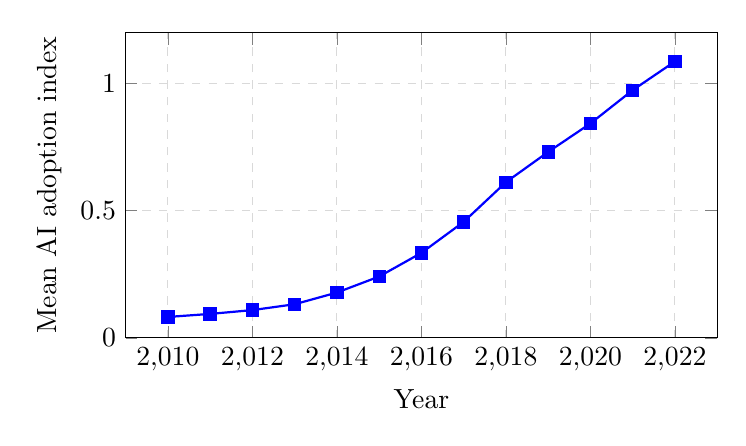
\begin{tikzpicture}
\begin{axis}[
  width=0.75\textwidth,
  height=0.45\textwidth,
  xlabel={Year},
  ylabel={Mean AI adoption index},
  xmin=2009, xmax=2023,
  ymin=0, ymax=1.2,
  xtick={2010,2012,2014,2016,2018,2020,2022},
  legend pos=north west,
  grid=major,
  grid style={dashed,gray!30},
]
\addplot[blue, thick, mark=square*, mark size=2pt] coordinates {
  (2010, 0.082) (2011, 0.094) (2012, 0.109) (2013, 0.132)
  (2014, 0.178) (2015, 0.241) (2016, 0.334) (2017, 0.456)
  (2018, 0.612) (2019, 0.731) (2020, 0.843) (2021, 0.974) (2022, 1.087)
};
\end{axis}
\end{tikzpicture}
\caption{AI Adoption Trend among Sample Firms, 2010--2022}
\label{fig:aitrend}
\begin{minipage}{0.86\textwidth}
\footnotesize
Notes: The figure plots the annual mean AI adoption index across the 10,563 firm-year observations. The index is the log of one plus the frequency of AI-related terms normalized by annual report length. The upward trend reflects growing AI diffusion, particularly accelerating after 2016 with advances in deep learning.
\end{minipage}
\end{figure}

\begin{figure}[H]
\centering
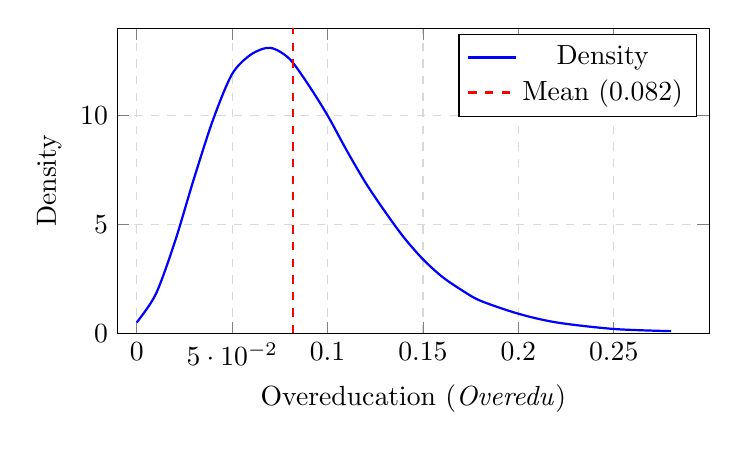
\begin{tikzpicture}
\begin{axis}[
  width=0.75\textwidth,
  height=0.45\textwidth,
  xlabel={Overeducation (\(\Overedu\))},
  ylabel={Density},
  xmin=-0.01, xmax=0.30,
  ymin=0, ymax=14,
  xtick={0, 0.05, 0.10, 0.15, 0.20, 0.25},
  grid=major,
  grid style={dashed,gray!30},
]
\addplot[blue, thick, smooth] coordinates {
  (0.00, 0.5) (0.01, 1.8) (0.02, 4.2) (0.03, 7.1) (0.04, 9.8)
  (0.05, 11.9) (0.06, 12.8) (0.07, 13.1) (0.08, 12.6) (0.09, 11.4)
  (0.10, 10.0) (0.11, 8.4) (0.12, 6.9) (0.13, 5.6) (0.14, 4.4)
  (0.15, 3.4) (0.16, 2.6) (0.17, 2.0) (0.18, 1.5) (0.20, 0.9)
  (0.22, 0.5) (0.25, 0.2) (0.28, 0.1)
};
\addplot[red, dashed, thick] coordinates {(0.082, 0) (0.082, 14)};
\legend{Density, Mean (0.082)}
\end{axis}
\end{tikzpicture}
\caption{Distribution of Firm-Level Overeducation, Pooled Sample}
\label{fig:overedudist}
\begin{minipage}{0.86\textwidth}
\footnotesize
Notes: Kernel density of $\Overedu$ across the 10,563 firm-year observations. The red dashed line marks the sample mean (0.082). The distribution is right-skewed with a mode near 0.07, consistent with moderate overeducation in most firms and a tail of highly mismatched firms.
\end{minipage}
\end{figure}

\end{appendices}

\end{document}
